\chapter{Doświadczenie}
\label{cha:dos}
W ramach niniejszej pracy dyplomowej przeprowadzono doświadczenie polegające na porównaniu autorskiego algorytmu klasyfikacji (stworzonego w ramach pracy inżynierskiej pt. „Wykorzystanie algorytmów genetycznych w systemach wykrywania intruzów w sieciach komputerowych”~\cite{Blyszcz2022}) wraz z:
\begin{itemize}
    \item algorytmami klasyfikacji danych dwuklasowych dostępnymi w środowisku Microsoft Azure,
    \item algorytmem DANet~\cite{Danet, Chen2022}
\end{itemize}
Algorytmy opisano w kolejnych podrozdziałach.\ Doświadczenie przeprowadzono w następujących etapach:
\begin{enumerate}
    \item Określenie założeń technicznych
    \item Wybór danych i algorytmów klasyfikacji
    \item Konfiguracja programistycznego środowiska badawczego
    \item Utworzenie doświadczenia
    \item Przeprowadzenie badań
    \item Analiza wyników.
\end{enumerate}


\section{Metodologia badawcza}
\label{sec:met}
W celu oceny jakości algorytmów klasyfikacji określono następujący protokół metodologii badawczej, który został przedstawiony w \refsource{tabeli}{tab:met-bad}.\ Na początku zdefiniowano problem badawczy, określono do niego pytania badawcze oraz postawiono przewidywane hipotezy.
\vfill
\pagebreak
\begin{table}[H]
    \centering
    \captionsource{Metodologia badawcza}{Opracowanie własne}
    \begin{tabular}{|L{\textwidth}|}
        \hline
        \textbf{Problem badawczy:}                                                                                                                     \\
        Czy algorytm klasyfikacji danych utworzony w ramach pracy inżynierskiej może konkurować z rozwiązaniami dostępnymi w środowiskach komercyjnych? \\ \hline

        \textbf{Pytania badawcze:}                                                                                                                     \\
        \begin{enumerate}
            \item Czy algorytm jest konkurencyjny pod względem wybranych metryk:
            \begin{itemize}
                \item dokładność algorytmu
                \item czas działania
                \item precyzja
                \item czułość
                \item F1
                \item AUC?
            \end{itemize}
        \end{enumerate}                                                                                                                                \\ \hline

        \textbf{Hipotezy:}                                                                                                                             \\
        \begin{enumerate}
            \item Nie ma istotnej różnicy pomiędzy wynikami próby testowej i treningowej nr. 1.
            \item Nie ma istotnej różnicy pomiędzy wynikami prób testowych.
            \item Wynik dopasowania algorytmów w \textit{Próbie 1} nie przekracza dolnej granicy przedziału ufności dla próby testowej
        \end{enumerate}                                                                                                                                \\ \hline
    \end{tabular}
    \label{tab:met-bad}
\end{table}


\section{Założenie techniczne}

Dane prezentowane w \refsource{Tabeli}{tab:technical} określają podstawowe założenia techniczne przyjęte w trakcie wykonywania analizy porównawczej.\ Dane te dotyczą między innymi środowiska, w którym wykonane było doświadczenie.\ Dodatkowo uwzględniono zestaw danych oraz biblioteki użyte w trakcie tworzenia doświadczenia.

\begin{table}[H]
    \centering
    \captionsource{Założenia techniczne pracy dyplomowej}{Opracowanie własne}
    \label{tab:technical}
    \begin{tabular}{|l|l|}
        \hline
        \textbf{Środowisko uruchomieniowe}              & Machine Learning Studio\cite{azureml} \\ \hline
        \textbf{Język programowania}                    & Python 3.x                            \\ \hline
        \multirow{3}*{\textbf{Wykorzystane biblioteki}} & scikit-learn~\cite{scikit-learn}      \\
        \cline{2-2}
        & Numpy~\cite{Harris2019}               \\
        \cline{2-2}
        & Pandas~\cite{pandas, McKinney2010}    \\
        \hline
        \textbf{Wykorzystane dane}                      & CICDS2017~\cite{cicds2017kaggle}      \\
        \hline
    \end{tabular}
\end{table}


\section{Dane}
\label{sec:data}
Zbiór danych został przygotowany przez Kanadyjski Instytut Cyberbezpieczeństwa działający przy Uniwersytecie Nowy Brunszwik.\ Został wykonany za pomocą narzędzia CICFlowMeter
~\cite{Ahlashkari2022}.\ Zbiór zawiera 79 cech ruchu sieciowego, do których zaliczyć można:
\begin{enumerate}
    \item etykietę,
    \item czas trwania przesyłu,
    \item minimalną długość pakietu zwrotnego,
    \item maksymalną długość pakietu zwrotnego,
    \item port docelowy,
    \item długość pakietów.
\end{enumerate}
Zbiór pozwala na określenie czy ruch sieciowy jest życzliwy \trans{ang. BENING}, czy nieżyczliwy (różne możliwe formy ataku na sieć).\ Dodatkowo dane zostały podzielone na pięć dni roboczych: poniedziałek 3.07.2017 - piątek 7.07.2017.\ Dane z poniedziałku zawierają jedynie ruch życzliwy.\ W pozostałe dni zostały zasymulowane ataki na sieć komputerową~\cite{Blyszcz2022, unbkaggle}.


\section{Algorytmy wykorzystane w doświadczeniu}
\label{sec:alg}
W trakcie eksperymentu zastosowano różne algorytmy klasyfikacji danych, by móc ocenić jakość autorskiego rozwiązania Gausian Naive Bayes - with GA. Do porównania wykorzystano następujące algorytmy takie jak:
\begin{enumerate}
    \item Two-Class Support Vector Machine
    \item Two-Class Boosted Decision Tree
    \item Two-Class Decision Forest
    \item Two-class Neural Network
    \item Two-Class Average Perceptron
    \item DANet.
\end{enumerate}
Algorytmy 1 - 5 są dostępne na platformie Microsoft Azure, natomiast algorytm 6 to rozwiązanie udostępnione przez jednego z autorów pracy na platformie Github~\cite{Danet}.

Charakterystyczną cechą tych algorytmów jest klasyfikacja ukierunkowana na 2 kategorie wejściowe.\ W tym wypadku są to kategorie ruchu sieciowego:
\begin{itemize}
    \item \textbf{BENIGN} \trans{pl. życzliwy},
    \item \textbf{OTHER} \trans{pl. inne}, gdzie inne to pozostałe typy ruchu sieciowego.
\end{itemize}

W kolejnych podrozdziałach pokrótce scharakteryzowano zastosowane rozwiązania.

\subsection{Two-Class Support Vector Machine}\label{subsec:svm}
Algorytm SVM ma za zadanie znaleźć hiperpłaszczyznę w przestrzeni K-wymiarowej (gdzie K - liczba cech), która rozdziela zbiory punktów odpowiadające różnym klasom.\ W pierwszej kolejności SVM szuka separatora między klasami, a następnie przekształca się dane w taki sposób, by móc przekształcić separator w hiperpłaszczyznę~\cite{IBM}.\ Sposób działania został zobrazowany za pomocą \refsource{wykresów}{fig:svm}.

\begin{figure}[H]
    \begin{subfigure}[m]{0.45\textwidth}
        \centering
        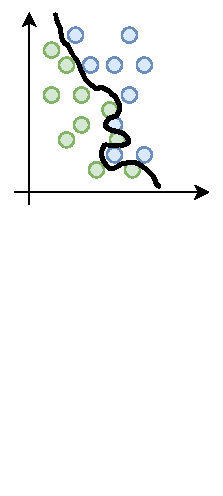
\includegraphics[width=\textwidth]{images/svm_2}
    \end{subfigure}
    \hfill
    \begin{subfigure}[m]{0.45\textwidth}
        \centering
        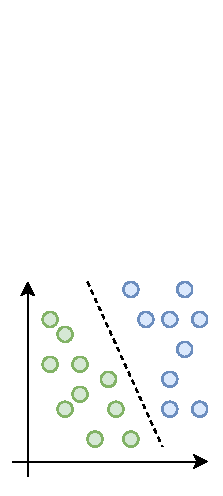
\includegraphics[width=\textwidth]{images/svm_1}
    \end{subfigure}
    \captionsource{Schemat SVM}{\cite{Statsoft}}
    \label{fig:svm}
\end{figure}

Implementacja algorytmu w Azure Machine Learning zostałą przedstawiona na \refsource{rysunku}{fig:svm-pipe}.

\begin{figure}[H]
    \centering
    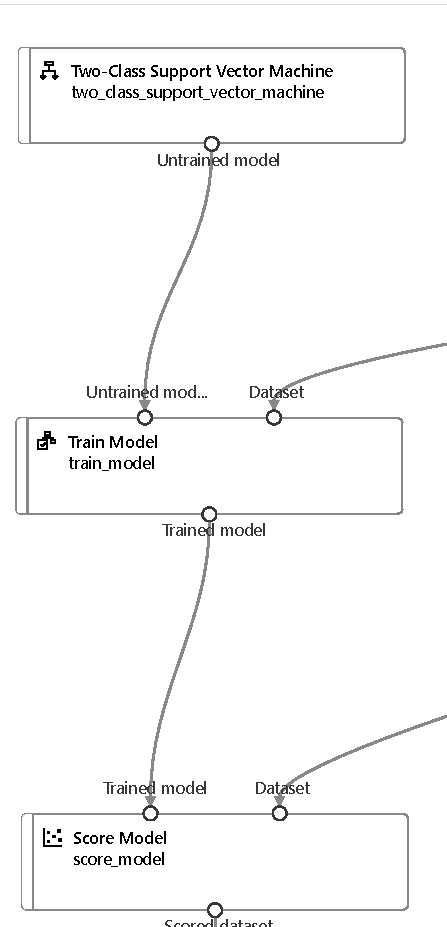
\includegraphics[width=0.4\textwidth]{images/svm_pipe}
    \captionsource{Potok zadań dla modelu \textit{Two-Class Support Vector Machine}}{Opracowanie własne}
    \label{fig:svm-pipe}
\end{figure}

Jest to część potoku, która obrazuje schemat działania procesu trenowania i sprawdzania algorytmu.\ Pierwszy kafelek obrazuje model SVM, który jest podłączony do elementu odpowiadającego za trening modelu.\ Do tego samego miejsca sa podłączone dane treningowe.\ Po wykonaniu zadania trenowania następuje przejście do zadania oceniającego model.\ Do tego zadania podłączone są dane testowe.\ Przy pomocy danych testowych następuje ewaluacja modelu.\ Wyniki ewaluacji są przekazywane do zbiorczej tabeli.

\subsection{Two-Class Boosted Decision Tree}
Jest to algorytm drzewa decyzyjnego oparty o algorytm LightGBM.\ Dzięki zastosowaniu takiego podejścia algorytm działa szybciej oraz ma mniejszą złożoność obliczeniową.\ Algorytm ten działa na zasadzie doboru odpowiedniego liścia, zamiast jak w przypadku klasycznych algorytmów opartych na drzewie, wyboru odpowiedniej warstwy~\cite{LightGBM}.\ Sposób podejścia liściastego został ukazany na \refsource{schemacie}{fig:leaf}.\ Model wykorzystywany w Azure ML został ukazany na \refsource{rysunku}{fig:dt-pipe}.
\vfill
\pagebreak
\begin{figure}[H]
    \begin{subfigure}[m]{\textwidth}
        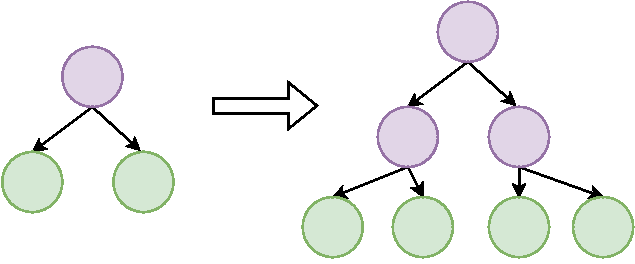
\includegraphics[width=\textwidth]{images/level-wise}
    \end{subfigure}
    \begin{subfigure}[m]{\textwidth}
        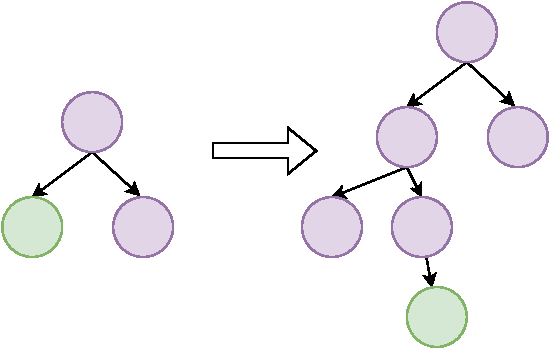
\includegraphics[width=\textwidth]{images/leaf-wise}
    \end{subfigure}
    \captionsource{Sposób działania algorytmu}{\cite{LightGBM}}
    \label{fig:leaf}
\end{figure}

\begin{figure}[H]
    \centering
    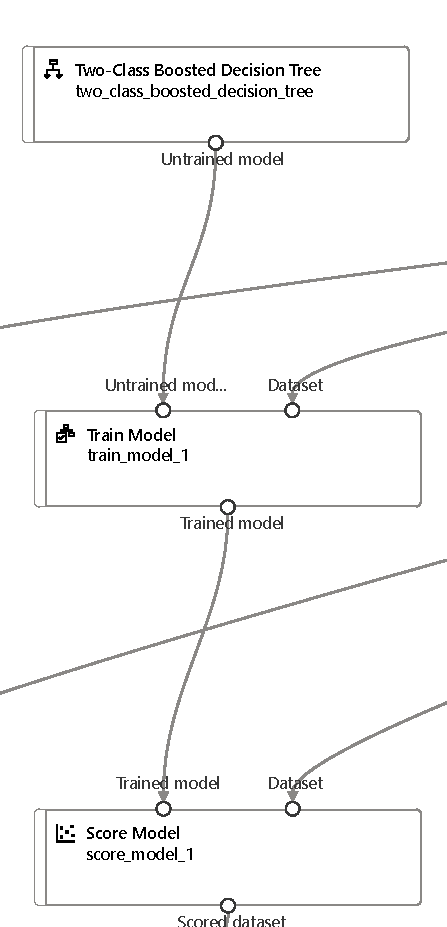
\includegraphics[width=0.4\textwidth]{images/dt_pipe}
    \captionsource{Potok zadań dla modelu \textit{Two-Class Boosted Decision Tree}}{Opracowanie własne}
    \label{fig:dt-pipe}
\end{figure}

Potok jest zbudowany analogicznie do potoku opisanego w \refsource{podsekcji}{subsec:svm}.\ Do bloku treningowego został podłączony model wzmocnionego drzewa decyzyjnego.

\subsection{Two-Class Decision Forest}
Las decyzyjny to algorytm, którego wynik opiera się o agregację wyników wielu drzew decyzyjnych.\ Uzyskanie wyniku zależy od algorytmu trenowania lasu.\ Przykładowo w klasyfikacji losowym lasem wieloklasowym \trans{ang. Multi-class random forest classification}, każde drzewo głosuje na jedną klasę.\ Klasa, która zostanie wybrana większością głosów, zostaje uznana za wynikową~\cite{Google}.\ Model wykorzystany w Azure ML pokazano na \refsource{modelu}{fig:df-pipe}.

\begin{figure}[H]
    \centering
    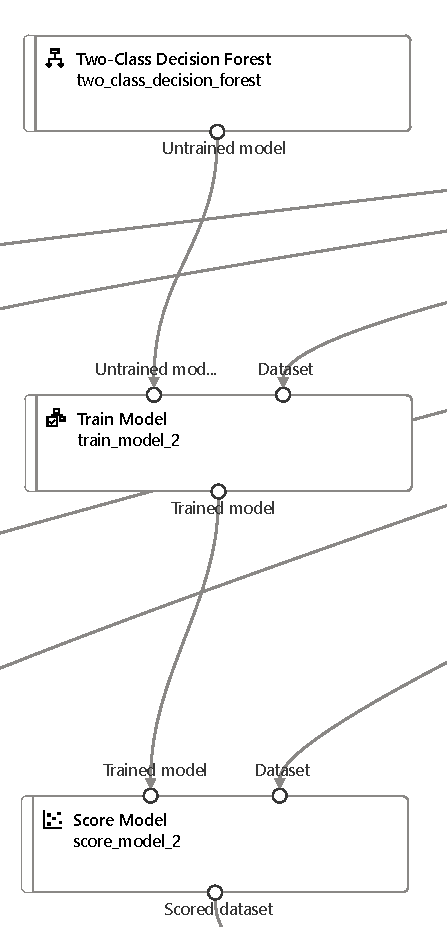
\includegraphics[width=0.4\textwidth]{images/df_pipe}
    \captionsource{Potok zadań dla modelu \textit{Two-Class Decision Forest}}{Opracowanie własne}
    \label{fig:df-pipe}
\end{figure}

Potok został zbudowany analogicznie do potoku opisanego w \refsource{podsekcji}{subsec:svm}.\ Do bloku treningowego został podłączony model lasu decyzyjnego.

\subsection{Two-class Neural Network}
Jest to sieć neuronowa, która składa się z warstwy wejściowej, trzech warstw ukrytych (każda posiada po 100 węzłów), oraz z warstwy wyjściowej.\ Przykładowa sieć neuronowa została zobrazowana na \refsource{schemacie}{fig:neural-network}.\ Moduł wykorzystany w Azure ML ukazano na \refsource{rysunku}{fig:nn-pipe}.

\begin{figure}[H]
    \centering
    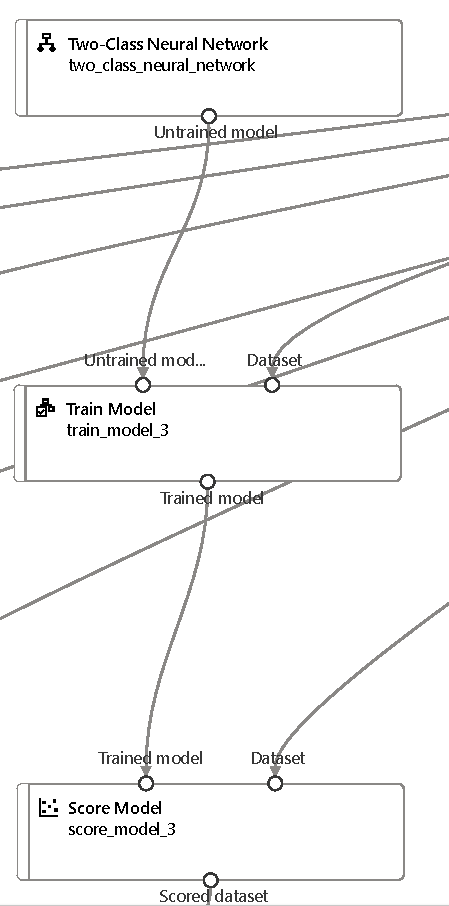
\includegraphics[width=0.4\textwidth]{images/nn_pipe}
    \captionsource{Potok zadań dla modelu \textit{Two-Class Neural Network}}{Opracowanie własne}
    \label{fig:nn-pipe}
\end{figure}

Potok jest zbudowany analogicznie do potoku opisanego w \refsource{podsekcji}{subsec:svm}.\ Do bloku treningowego został podłączony model sieci neuronowej.

\subsection{Two-Class Average Perceptron}
Jest to najprostsza odmiana sieci neuronowej, czyli pojedynczy perceptron, który jest matematycznym modelem neuronu.\ Składa się on z \textit{n} wejść, takiej samej ilości wag, progu $\Theta$, sumatora, funkcji aktywującej i wyjścia.\ Został zobrazowany na \refsource{schemacie}{fig:neuron}.\ Może służyć za prosty klasyfikator binarny albo za regresor.\ Model wykorzystany w Azure ML ukazano na \refsource{zdjęciu}{fig:ap-pipe}.

\begin{figure}[H]
    \centering
    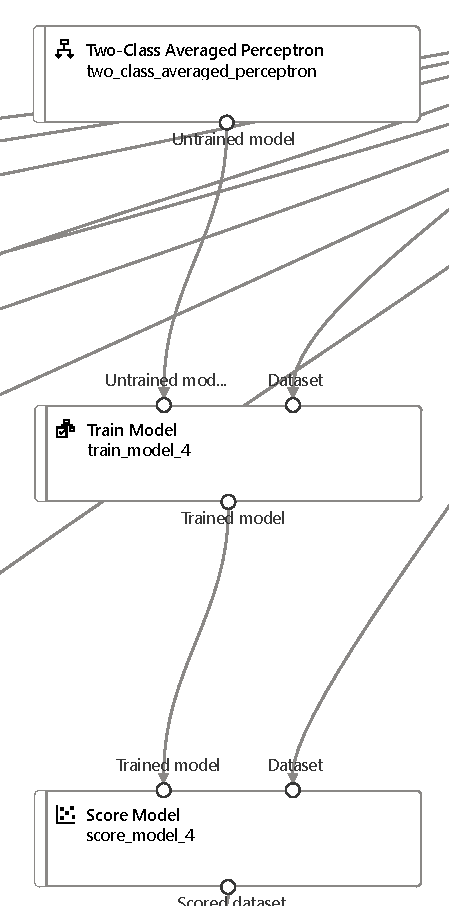
\includegraphics[width=0.4\textwidth]{images/ap_pipe}
    \captionsource{Potok zadań dla modelu \textit{Two-Class Average Perceptron}}{Opracowanie własne}
    \label{fig:ap-pipe}
\end{figure}

Potok jest zbudowany analogicznie do potoku opisanego w \refsource{podsekcji}{subsec:svm}.\ Do bloku treningowego został podłączony model klasycznego perceptronu.

\subsection{Gausian Naive Bayes - with GA}
Algorytm ten polega na połączeniu algorytmu genetycznego (GA) wraz z klasyfikatorem naiwnym Bayesa wykorzystującego rozkład Gaussa (GNB).\ Zadaniem algorytmu genetycznego jest znalezienie najistotniejszych cech w zbiorze tabelarycznym.\ Poszukiwane cechy powinny pozwolić na zmniejszenie wymiarowości danych oraz na zmniejszenie kosztów obsługi samego klasyfikatora.\ Co może zostać uzyskane późniejszych etapach testowania, ze względu na zmniejszoną ilość danych wymaganych do przetworzenia.\ GA wykorzystywał w metodzie \textbf{fitness} algorytm GNB w celu określenia dopasowania danych.\ Zadaniem GNB było znalezienie najlepszej dostępnej kombinacji cech, które pozwalały na uzyskanie najlepszego dopasowania~\cite{Blyszcz2022}.\ Model wykorzystywany w Azure ML różni się od gotowych modeli tym, że dołączono do niego bibliotekę napisaną w języku Python, która zawiera kod wykorzystywany w pracy inżynierskiej autora~\cite{Suvres2023}.
\begin{figure}[H]
    \centering
    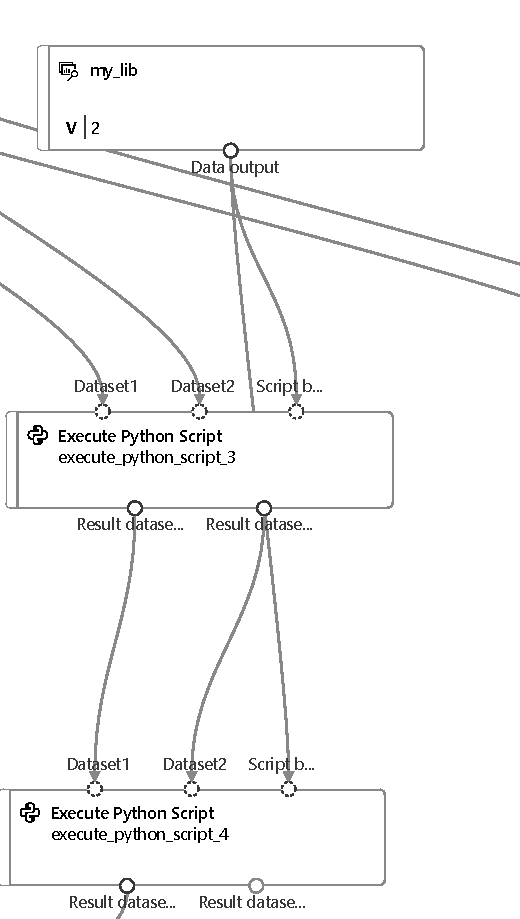
\includegraphics[width=0.4\textwidth]{images/ga_pipe}
    \captionsource{Potok zadań dla modelu \textit{Gaussian Naive Bayes - with GA}}{Opracowanie własne}
    \label{fig:ga-pipe}
\end{figure}

Potok został stworzony przy wykorzystaniu 3 głównych elementów:
\begin{itemize}
    \item \textbf{my\_lib} - jest to blok danych zawierających archiwum \textit{.zip}, w którym znajduje się biblioteka odpowiadająca za algorytm wykorzystywany w doświadczeniu,
    \item \textbf{Execute Python Script} (\textit{execute\_python\_script\_3}) blok wykonuję operację trenowania znajdującą się w bibliotece dołączonej do bloku.\ Do tego celu potrzeba było podłączyć dane testujące i treningowe do pierwszego bloku, by przekazać je dalej wraz z wytrenowanym modelem.
    \item \textbf{Execute Python Script} (\textit{execute\_python\_script\_4}) zadanie wykonuje operację testowania modelu, która znajduje się również w dołączonej bibliotece.\ Wynikiem obliczeń jest tabela z obliczonymi metrykami, która zostaje przekazana i dołączona do tabeli zbiorczej.
\end{itemize}

\subsection{DANet}
Twórcy tego algorytmu wprowadzają dodatkową warstwę abstrakcyjną o nazwie ,,\textit{Abstract Layer}''.\ Warstwy te budują sieć o nazwie ,,\textit{Deep Abstract Network}'' (DANet).\ Zadanie dodatkowych warstw jest grupowanie cech w skorelowanych zbiorach.\ Zbiory te budują sieć powiązań między sobą w formie sieci semantycznej.\ Gdy sieć semantyczna jest zbudowana, to w ostatnim kroku wykonywana jest klasyfikacja w trzywarstwowej sieci perceptronów \trans{ang. Multilayer Perceptron network, MLP}~\cite{Chen2022, Danet}.\ Sposób działania przedstawiono na \refsource{schemacie}{fig:danet-abst}.\ Model znajdujący się z Azure ML został przedstawiony na \refsource{zdjęciu}{fig:danet-pipe}.

\begin{figure}[H]
    \hfill
    \begin{subfigure}[m]{\textwidth}
        \centering
        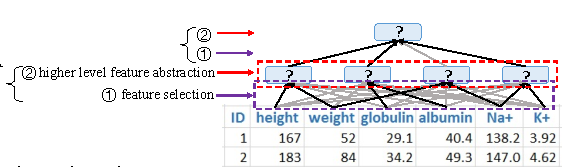
\includegraphics[width=\textwidth]{images/danet_1}
    \end{subfigure}
    \hfill
    \begin{subfigure}[m]{\textwidth}
        \centering
        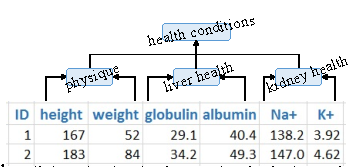
\includegraphics[width=\textwidth]{images/danet_2}
    \end{subfigure}
    \captionsource{Sposób działania DANet}{\cite{Chen2022}}
    \label{fig:danet-abst}
\end{figure}

\begin{figure}[H]
    \centering
    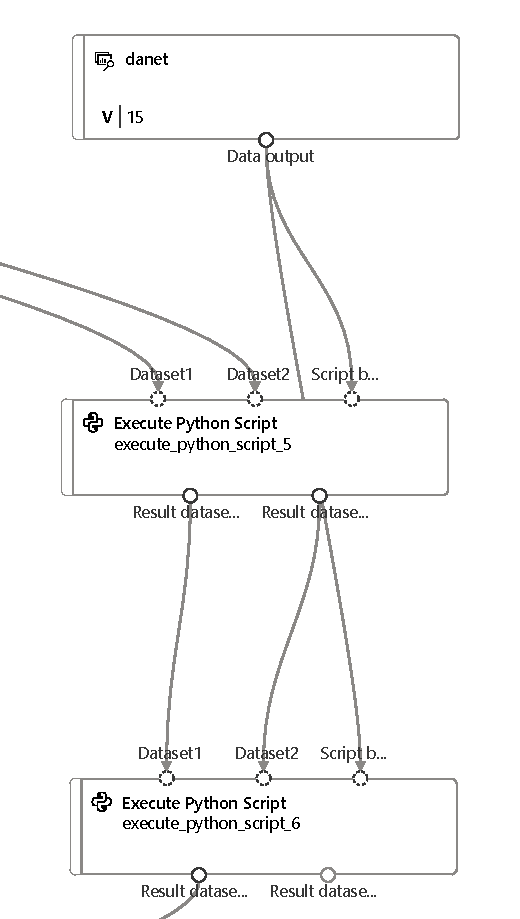
\includegraphics[width=0.4\textwidth]{images/danet}
    \captionsource{Potok zadań dla modelu \textit{DANet}}{Opracowanie własne}
    \label{fig:danet-pipe}
\end{figure}


\section{Programistyczne środowisko badawcze}
Analizę porównawczą algorytmów wykonano na platformie Microsoft Azure.\ Wykorzystano usługę Azure Machine Learning Studio.\ Wybrano to rozwiązanie, ponieważ umożliwia uniezależnienie obliczeń od komputera lokalnego.\ Dodatkowo, w łatwy sposób pozwala tworzyć skomplikowane potoki zadań, składające się z komponentów wielokrotnego użytku.\ Każdy komponent uruchamia się w środowisku odizolowanym od pozostałych operacji.\ Dzieje się tak dzięki wykorzystaniu wielowęzłowych klastrów obliczeniowych, bazujących na oprogramowaniu Docker.\ Klastry te mogą skalować się w zależności od potrzeb oraz dostępnej jednostki~\cite{MicrosoftLearn2023}.
\\ \\
Całe doświadczenie zostało odwzorowane w graficznym potoku narzędzia ,,\textit{Projektant}'' oraz przedstawione na \refsource{zdjęciu}{fig:pipeline}.

\begin{landscape}
    \centering
    \begin{figure}[H]
        \centering
        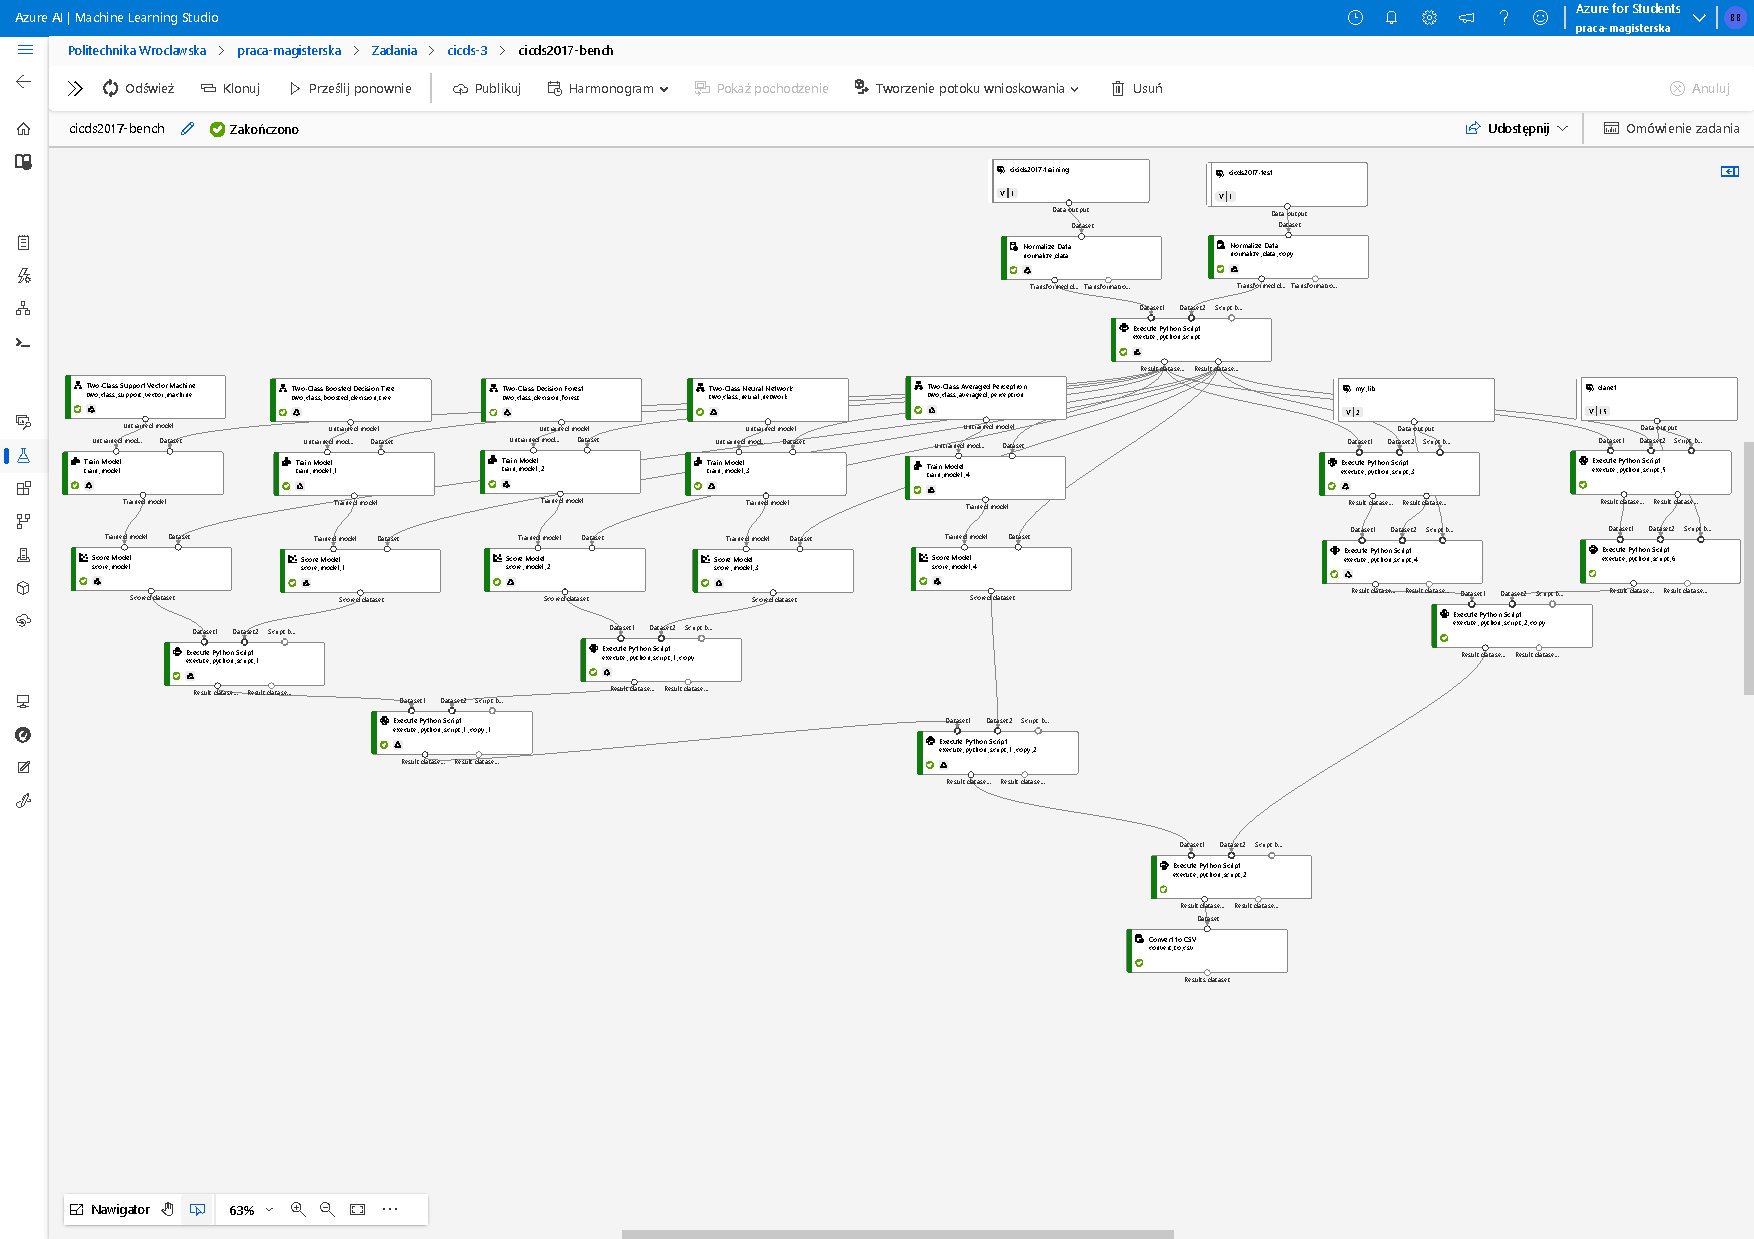
\includegraphics[height=0.9\textwidth]{images/pipeline}
        \captionsource{Potok zadań wykorzystywany w przeprowadzonym doświadczeniu}{Opracowanie własne}
        \label{fig:pipeline}
    \end{figure}
\end{landscape}

%%%%%%%%%%%%%%%%%%%%%%%%%%%%%%%%%%%%%%%%%%%%%%%%%%%%%%%%%%%%%%%%%%%%%%%%%%%%%%%%%%%%%%%%%%%%%%


\section{Przebieg eksperymentu}

,,\textit{Projektant}'', dostępny w Azure Machine Learning umożliwił utworzenie interaktywnego potoku zadań.\ Potok ten składa się z kilku części:
\begin{itemize}
    \item Przygotowanie i obróbka zbiorów danych
    \item Trenowanie oraz testowanie algorytmów klasyfikacji danych
    \item Utworzenie tabeli porównawczej dla wyników poszczególnych algorytmów (\refsource{obraz}{fig:pipeline}).
\end{itemize}

Poszczególne kroki przebiegu eksperymentu zostały opisane na kolejnych stronach.

\subsection{Przygotowanie danych}
W pierwszym kroku do normalizacji danych wykorzystano język Python oraz biblioteki Pandas i Numpy.\ Za pomocą wymienionych narzędzi, etykiety słowne zostają zamienione na wartości \textbf{0} i \textbf{1} oraz następuje zamiana wartości $[NaN, -inf, inf]$ na liczbę $0$.\ Cały proces został zobrazowany na \refsource{diagramie}{fig:norm}

\begin{figure}[H]
    \centering
    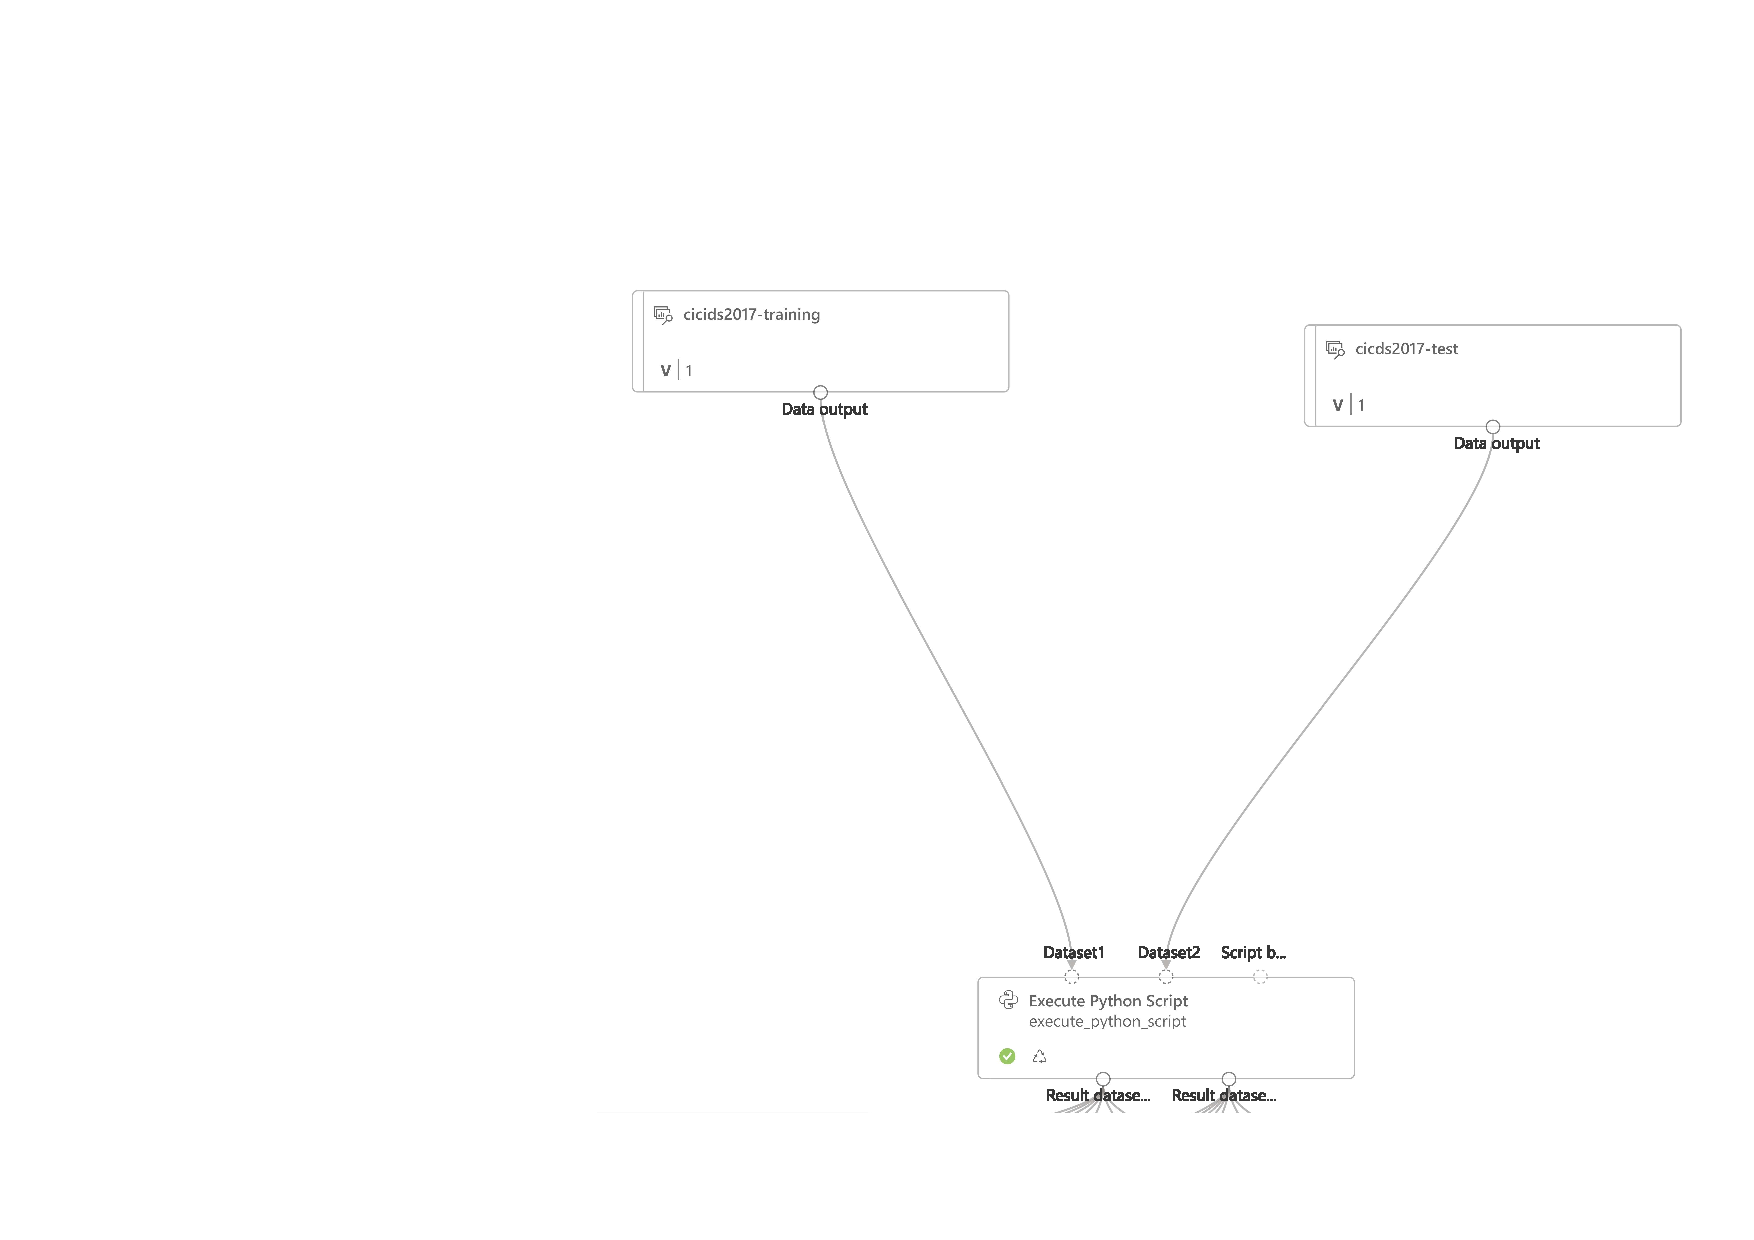
\includegraphics[width=0.6\textwidth]{images/data_pipe}
    \captionsource{Część potoku zajmująca się normalizacją danych}{Opracowanie własne}
    \label{fig:norm}
\end{figure}

\vfill
\pagebreak

\subsection{Trenowanie oraz testowanie algorytmów}
Kolejną grupą zadań widoczną w potoku są te związane z trenowaniem i testowaniem poszczególnych algorytmów opisanych w \refsource{rozdziale}{cha:dos}.\ Każdy test składa się 3 kafelek.\ W przypadku algorytmów dostarczonych wraz z platformą Azure ML są to:
\begin{itemize}
    \item \textbf{model klasyfikujący} - odpowiada za przygotowanie algorytmu klasyfikacyjnego
    \item \textbf{blok treningowy} - tworzy wytrenowany model, za pomocą połączonego zbioru danych
    \item \textbf{blok ewaluacyjny} - sprawdza wcześniej wytrenowany model za pomocą powiązanego zbioru danych.
\end{itemize}
Potok zadań wykorzystujący algorytmy dostarczone przez Microsoft Azure został ukazany na \refsource{schemacie}{fig:ms-pipe}

\begin{figure}[H]
    \centering
    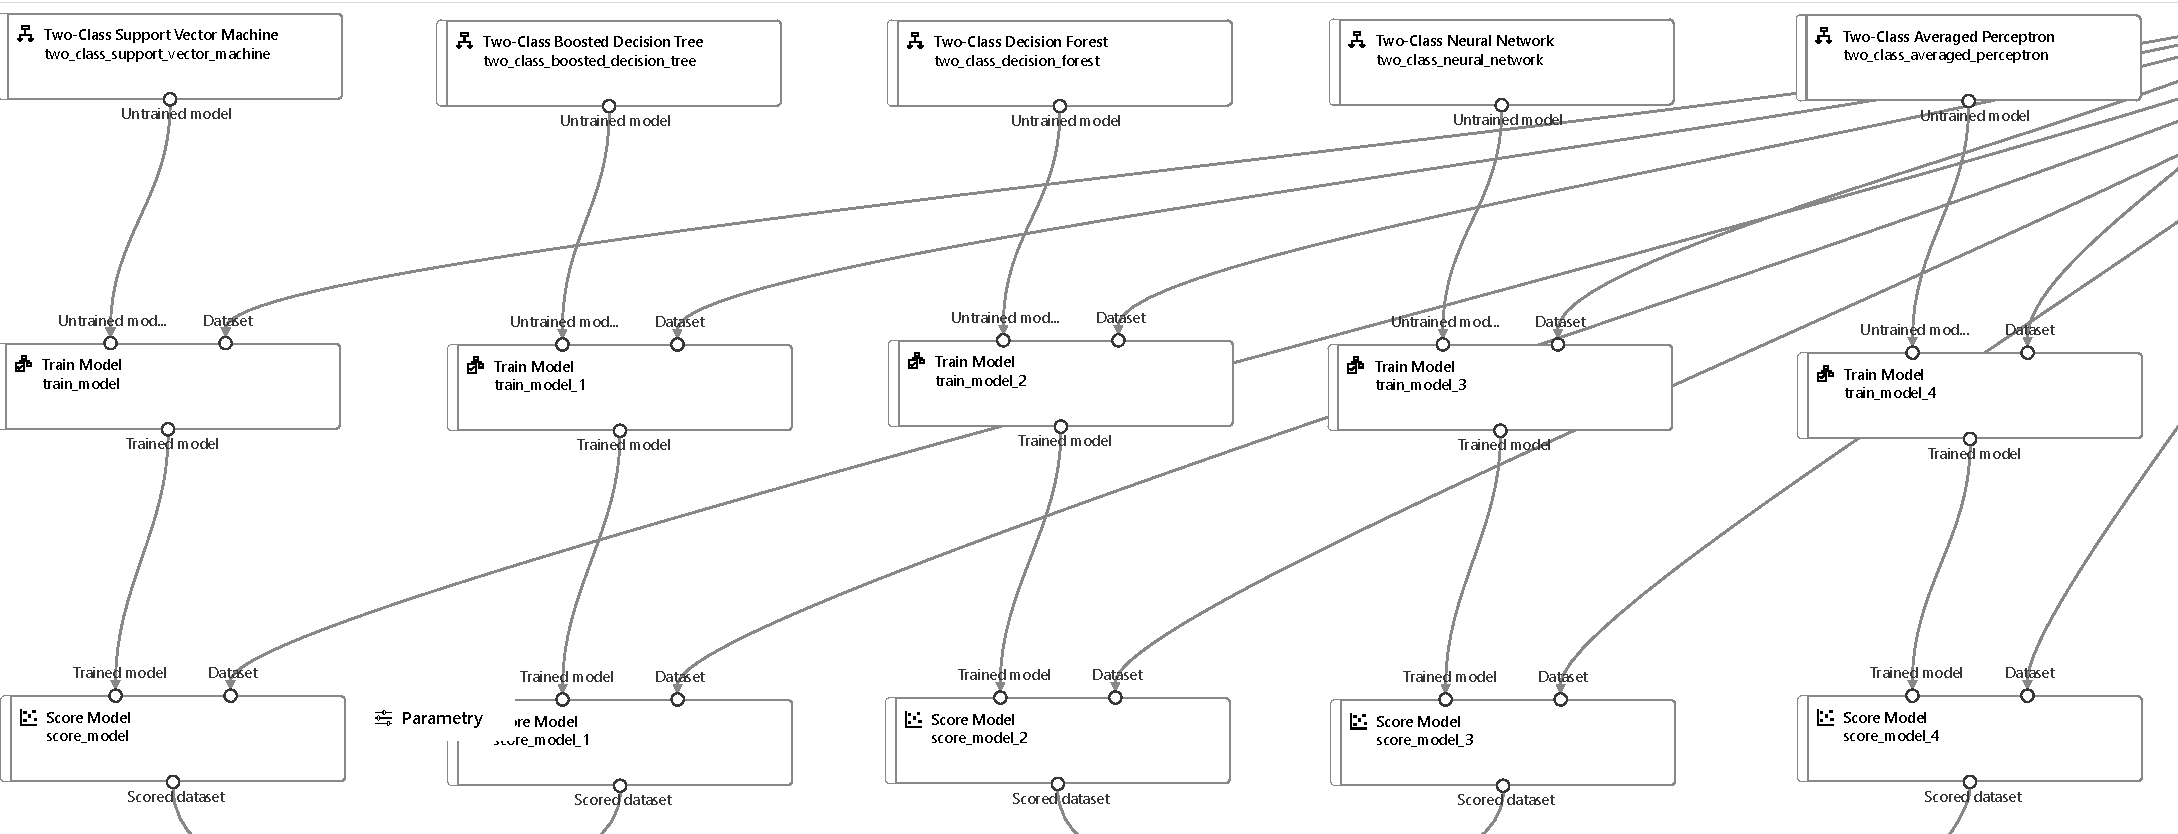
\includegraphics[width=\textwidth]{images/ms_pipe}
    \captionsource{Potok zadań dla algorytmów klasyfikacyjnych}{Opracowanie własne}
    \label{fig:ms-pipe}
\end{figure}

Algorytmy dostarczone w ramach pracy badawczej składają się z:
\begin{itemize}
    \item \textbf{biblioteka Python} - archiwum o rozszerzeniu \textbf{.zip}, które zawiera w sobie odpowiednie pliki napisane w języku Python
    \item \textbf{blok treningowy} - wykorzystuje dostarczoną bibliotekę do wytrenowania modelu oraz zapisania na platformie Azure najlepszego uzyskanego wyniku za pomocą powiązanego zbioru danych
    \item \textbf{blok ewaluacyjny} - wykorzystuje dostarczoną bibliotekę do ewaluacji algorytmu za pomocą połączonego zbioru danych
\end{itemize}

Potok zadań dla algorytmów niestandardowych został ukazany na \refsource{rysunku}{fig:au-pipe}

\begin{figure}[H]
    \centering
    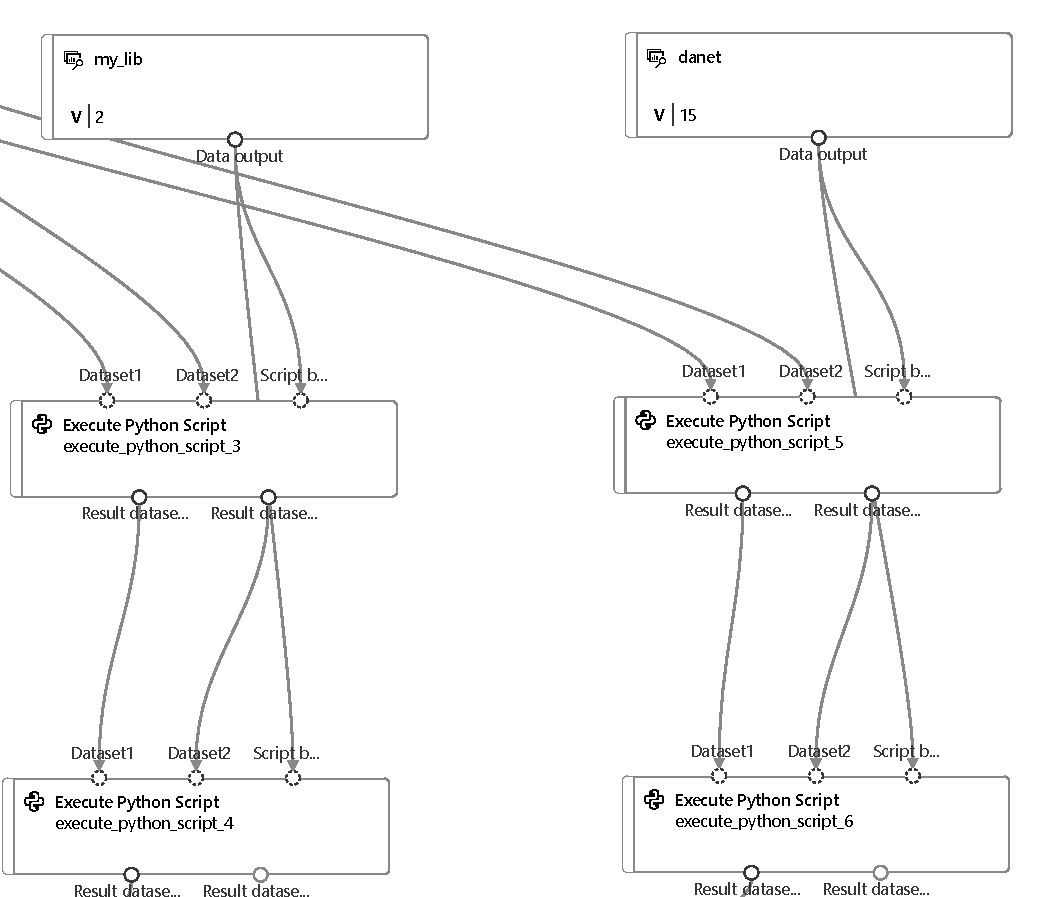
\includegraphics[width=0.8\textwidth]{images/au-pipe}
    \captionsource{Potok zadań dla algorytmów klasyfikacyjnych}{Opracowanie własne}
    \label{fig:au-pipe}
\end{figure}

\subsection{Utworzenie tabeli porównawczej}
Kolejną częścią zadań jest zebranie wyników poszczególnych algorytmów oraz połączenie ich w jedną całość.\ Wykorzystano do tego moduły języka Python, które zwracają przetworzone wyniki oraz łączą je w jedną tabelę zbiorczą, co pokazano na \refsource{rysunku}{fig:pipe-4}.

\begin{figure}[H]
    \centering
    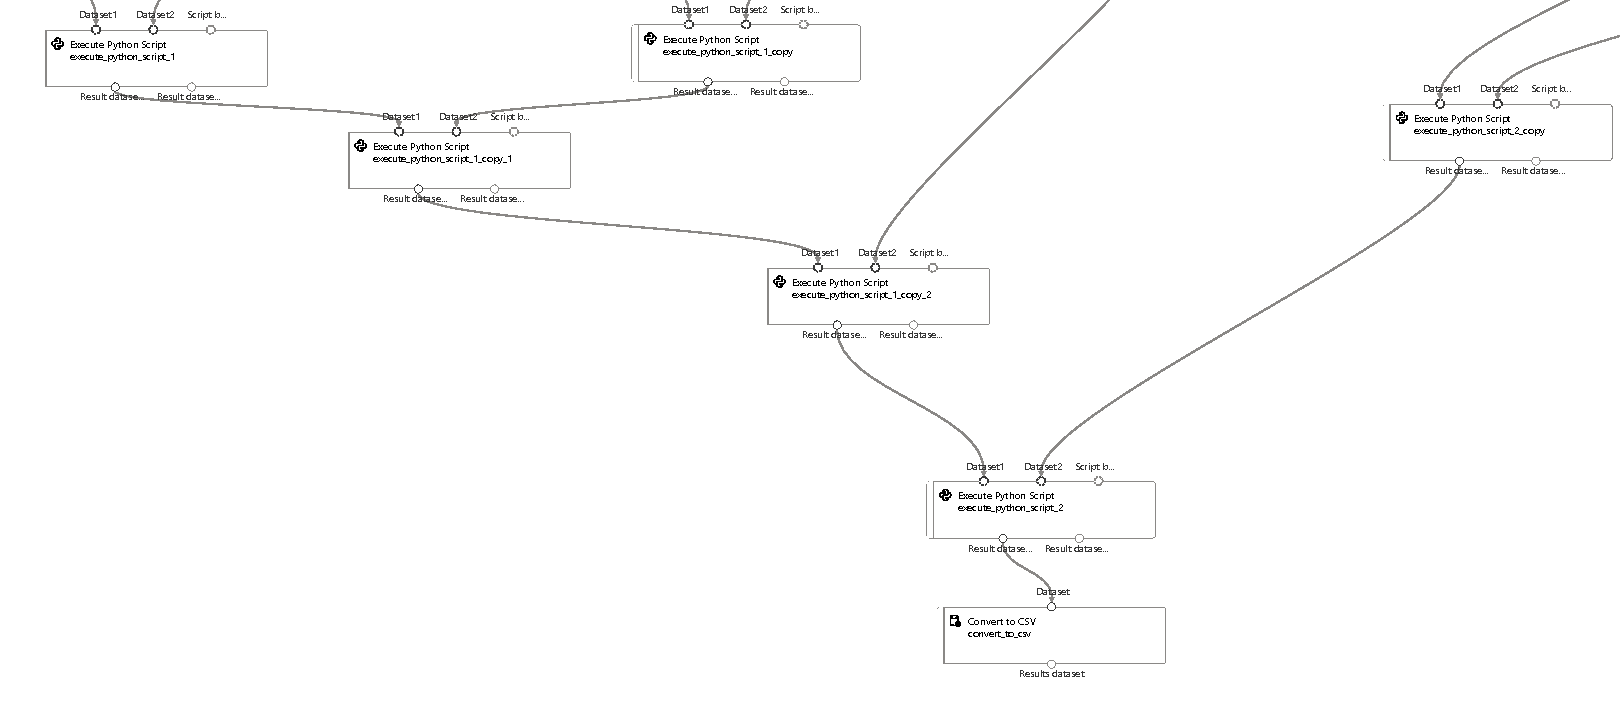
\includegraphics[width=\textwidth]{images/pipe-csv}
    \captionsource{Moduły odpowiedzialne za przetworzenie wyników}{Opracowanie własne}
    \label{fig:pipe-4}
\end{figure}

\subsection{Wyniki danych treningowych}
Aby zweryfikować działanie całego procesu klasyfikacji wykorzystano znormalizowane dane treningowe do wytrenowania oraz przetestowania działania algorytmów klasyfikacyjnych.\ Cały proces trwał ,,\textbf{1 dzień 10 godzin 55 minut 53 sekundy}''.\ Wyniki tych działań widać na \refsource{rysunku}{fig:predict-same}.\ Wykres przedstawia wyniki dla metryk klasyfikacyjnych jak:
\begin{itemize}
    \item dokładność
    \item precyzja
    \item czułość
    \item F1
    \item AUC.
\end{itemize}


Analizując wykres można zauważyć, że uzyskane wyniki znajdują się w przedziale $[94\%, 100\%]$ w każdej metryce co pokazuje jakość każdego z algorytmów, a także to, że algorytmy poradziły sobie niemal bezbłędnie w rozpoznawaniu ruchu sieciowego, na którym były uczone.\ Zbiór, który wykorzystano do trenowania oraz testowania danych zawierał w sobie 225805 wpisów z czego 97718 należało do klasy ,,\textbf{1}'', zaś 128087 należało do klasy ,,\textbf{0}''.\ Liczba klas wyjściowych wynosi \textit{2}, przez wzgląd na to, że jest to klasyfikacja binarna, która klasyfikuje dane jako \textit{1} albo \textit{0}.

\begin{table}[H]
    \centering
    \captionsource{Liczba elementów należących do danej klasy w zbiorze treningowym}{Opracowanie własne}
    \label{tab:trening-data-label}
    \begin{tabular}{|c|r|}
        \hline
        \textbf{Klasa} & \textbf{Liczba wystąpień} \\ \hline
        1              & 97718                     \\ \hline
        0              & 128027                    \\ \hline
        \textbf{Suma}  & 225805                    \\ \hline
    \end{tabular}
\end{table}

Bazując na tym zbiorze oraz uzyskanych wynikach udało się udowodnić poprawność działania procesu klasyfikacji wieloma algorytmami genetycznymi.

\begin{landscape}
    \vspace*{\fill}
    \begin{figure}[H]
        \centering
        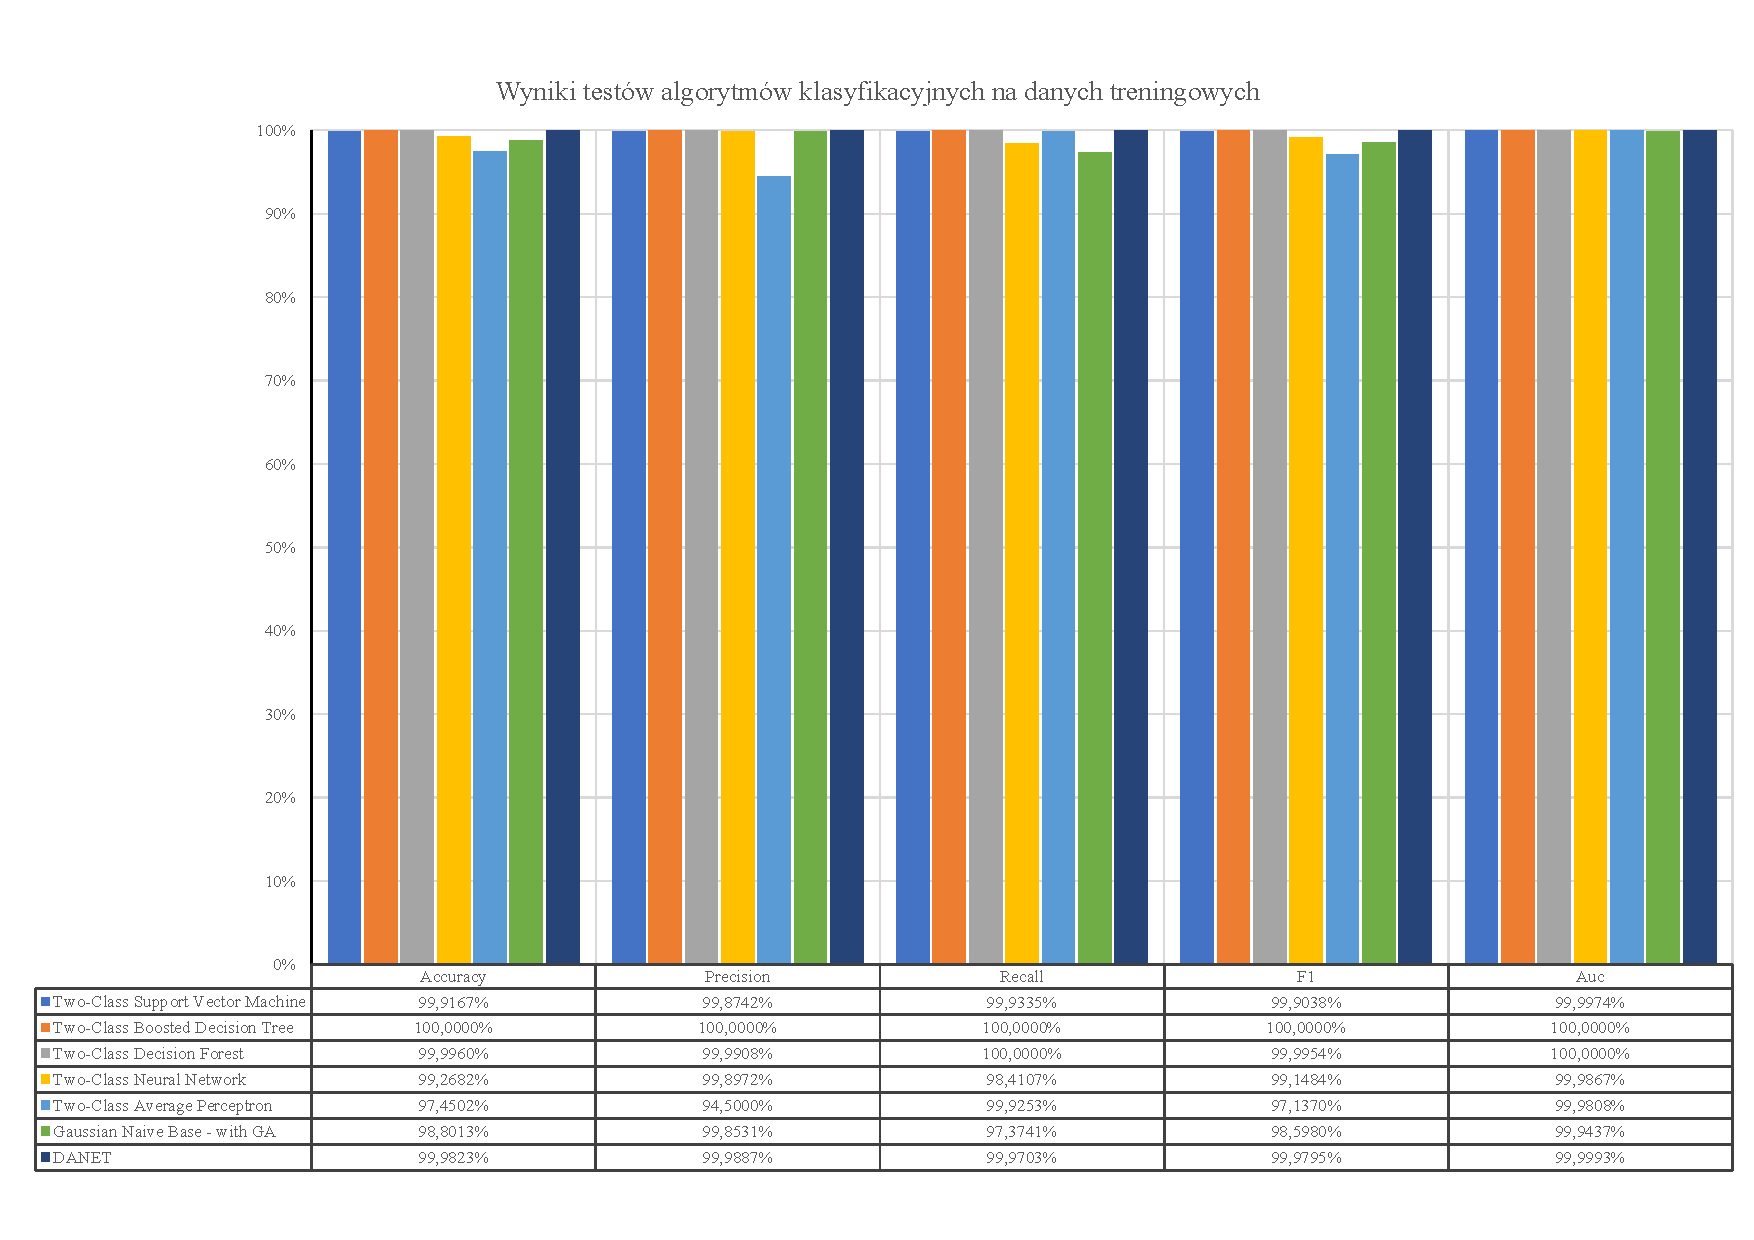
\includegraphics[height=0.8\textwidth]{images/predict_same}
        \captionsource{Wyniki testów algorytmów klasyfikacyjnych na danych treningowych}{Opracowanie własne}
        \label{fig:predict-same}
    \end{figure}
    \vfill
\end{landscape}


\section{Wyniki danych testowych}
Aby uzyskać realne wyniki podczas porównywania poszczególnych algorytmów zastosowano zbiór treningowy opisany w \refsource{tabeli}{tab:trening-data-label} oraz zbiór testowy, który zawierał 2273097 wpisów należących do klasy ,,\textbf{1}'' oraz 557646 wpisów należących do klasy ,,\textbf{0}''.\ Sumarycznie ilość wpisów wynosi: 2830743, co zostało pokazane w \refsource{tabel}{tab:res-test}.\ Pomiary testowe powtórzono 2 razy dzięki czemu uzyskano 3 próby badawcze.

\begin{table}[H]
    \centering
    \captionsource{Liczba elementów należących do danej klasy w zbiorze testowym}{Opracowanie własne}
    \label{tab:res-test}
    \begin{tabular}{|c|r|}
        \hline
        \textbf{Klasa} & \textbf{Liczba wystąpień} \\ \hline
        1              & 2273097                   \\ \hline
        0              & 557646                    \\ \hline
        \textbf{Suma}  & 2830743                   \\ \hline
    \end{tabular}
\end{table}

W analizie porównawczej algorytmów zastosowano następujące metryki klasyfikacji jak:
\begin{itemize}
    \item dopasowanie
    \item precyzja
    \item czułość
    \item F1
    \item AUC
\end{itemize}

Poniżej na \textbf{rysunkach:}~\textbf{\ref{fig:predict-result}},~\textbf{\ref{fig:predict-result2}},~\textbf{\ref{fig:predict-result3}} zostały przedstawione wyniki zbiorcze dla poszczególnych metryk.\ Dodatkowo przedstawiono również wynik pomiaru treningowego, który w większości przypadków jest wyższy od danych testowych.\ Co prawdopodobnie jest spowodowane różnicą w ilości danych testowych i treningowych.\ Dodatkowo w każdej kolumnie oznaczono kolorem zielonym najwyższy wynik dla danej metryki, a kolorem czerwonym najniższy wynik dla danej metryki.

\begin{landscape}
    \vspace*{\fill}
    \begin{figure}[H]
        \centering
        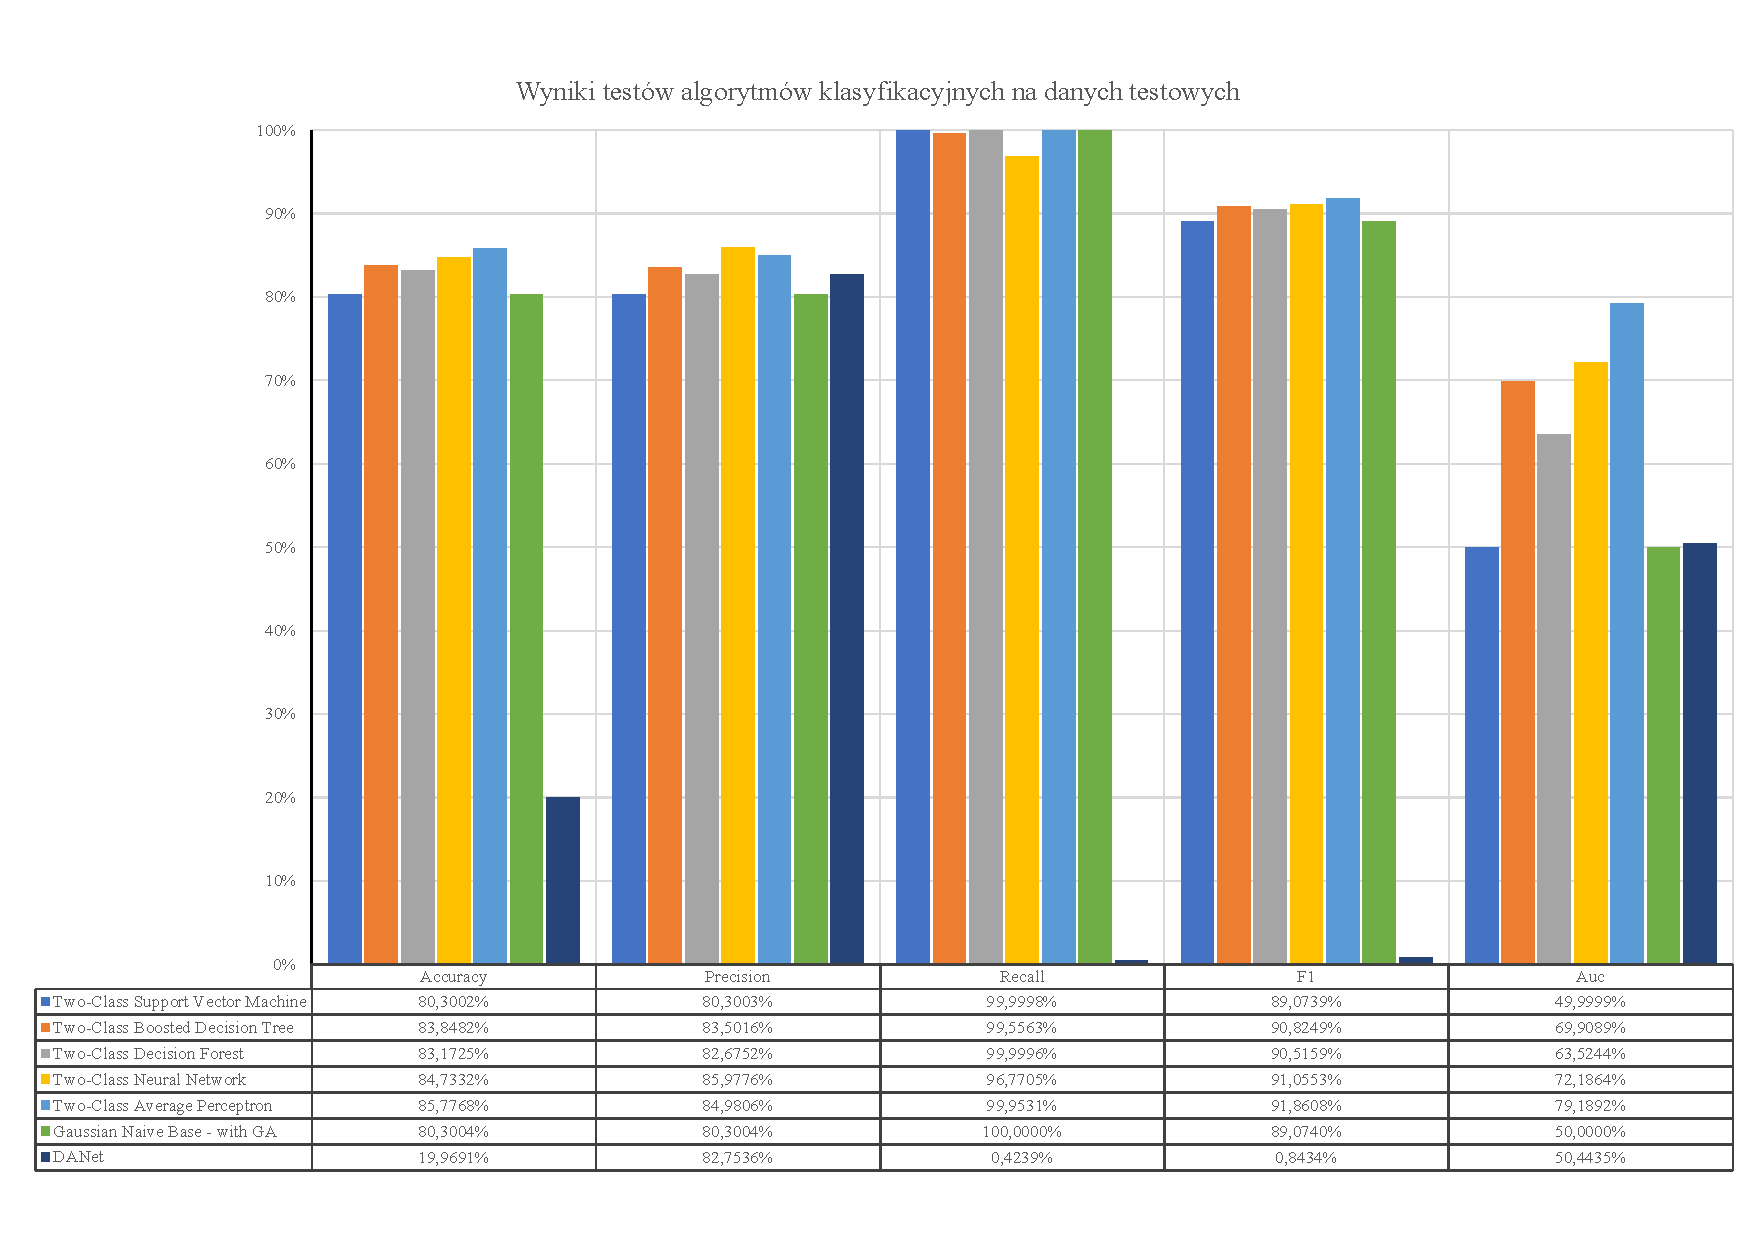
\includegraphics[height=0.8\textwidth]{images/predict_result}
        \captionsource{Wyniki testów algorytmów klasyfikacyjnych na danych testowych dla próby 1}{Opracowanie własne}
        \label{fig:predict-result}
    \end{figure}
    \vfill
\end{landscape}

\begin{landscape}
    \vspace*{\fill}
    \begin{figure}[H]
        \centering
        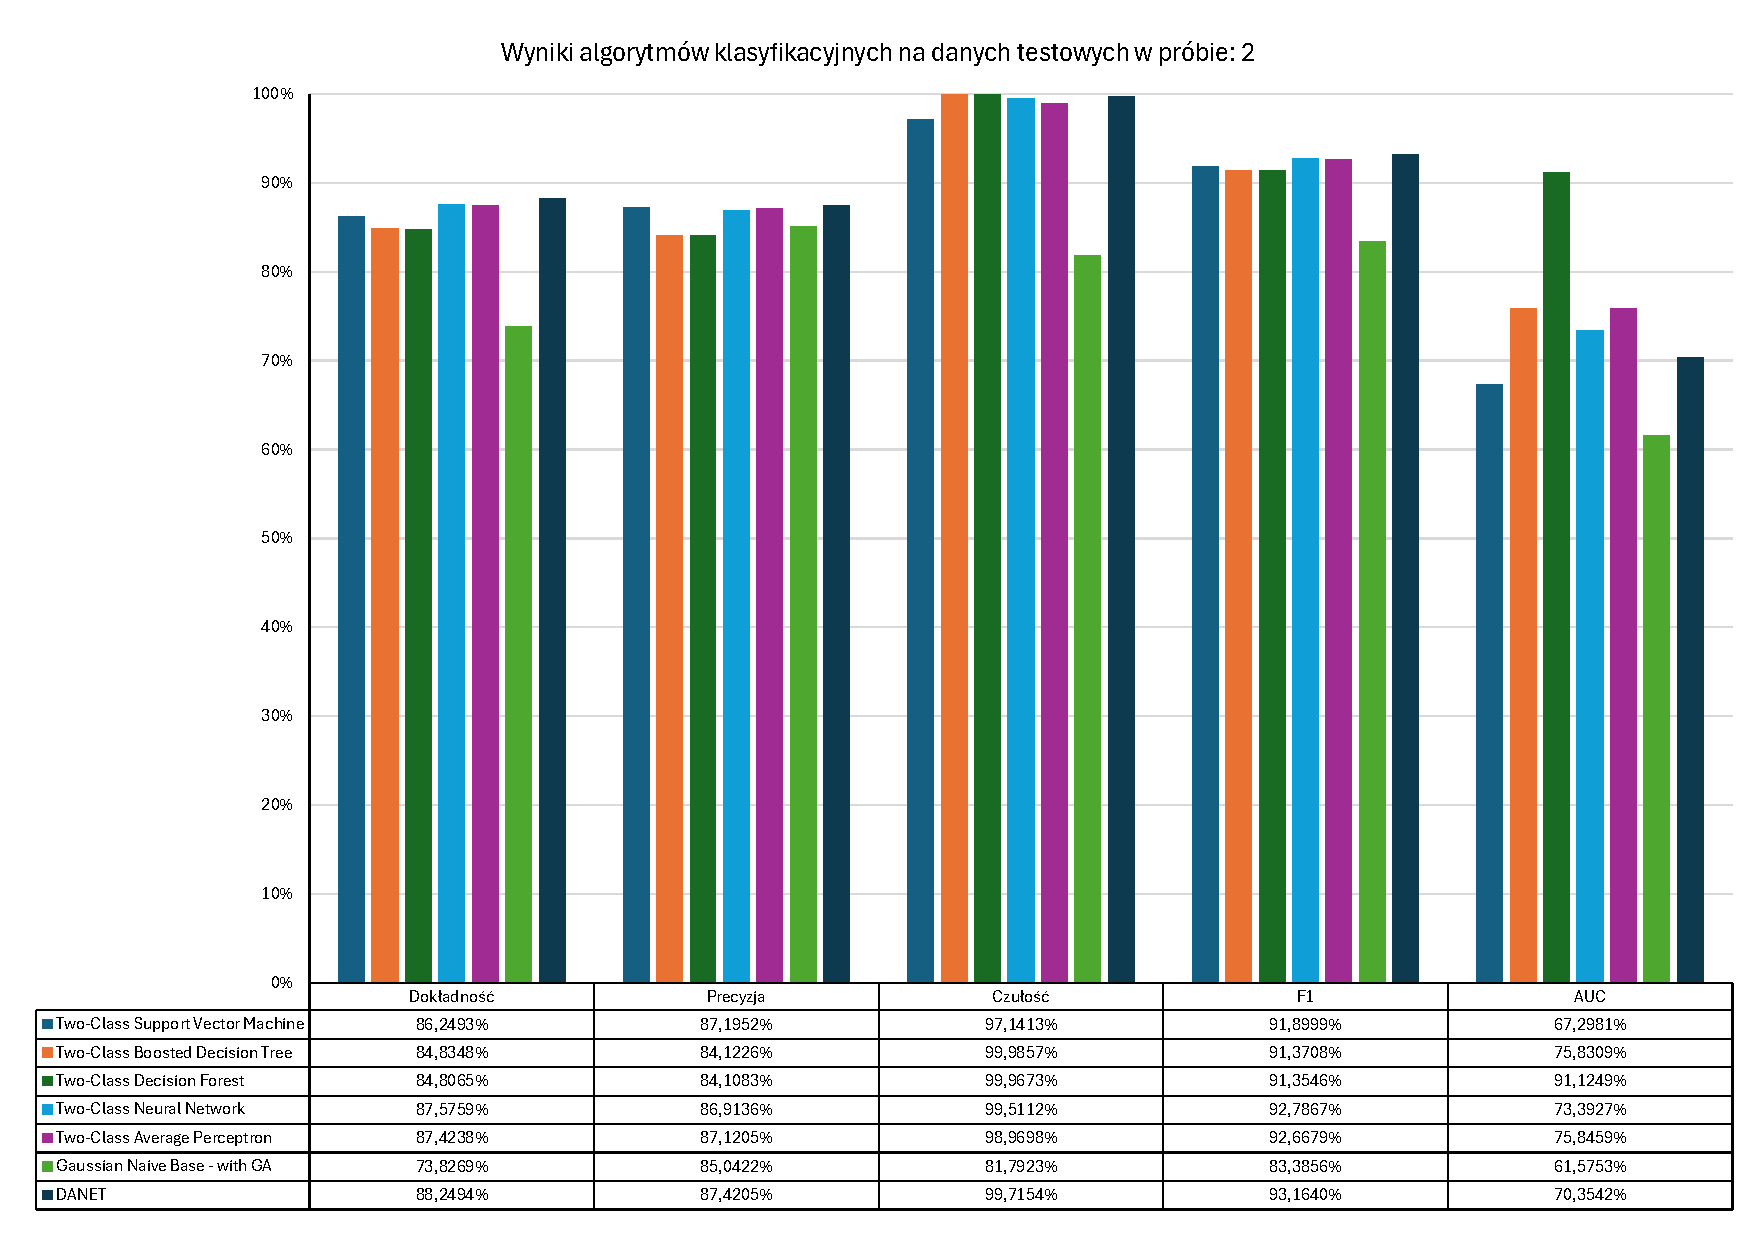
\includegraphics[height=0.8\textwidth]{images/predict_result_2}
        \captionsource{Wyniki testów algorytmów klasyfikacyjnych na danych testowych dla próby 2}{Opracowanie własne}
        \label{fig:predict-result2}
    \end{figure}
    \vfill
\end{landscape}

\begin{landscape}
    \vspace*{\fill}
    \begin{figure}[H]
        \centering
        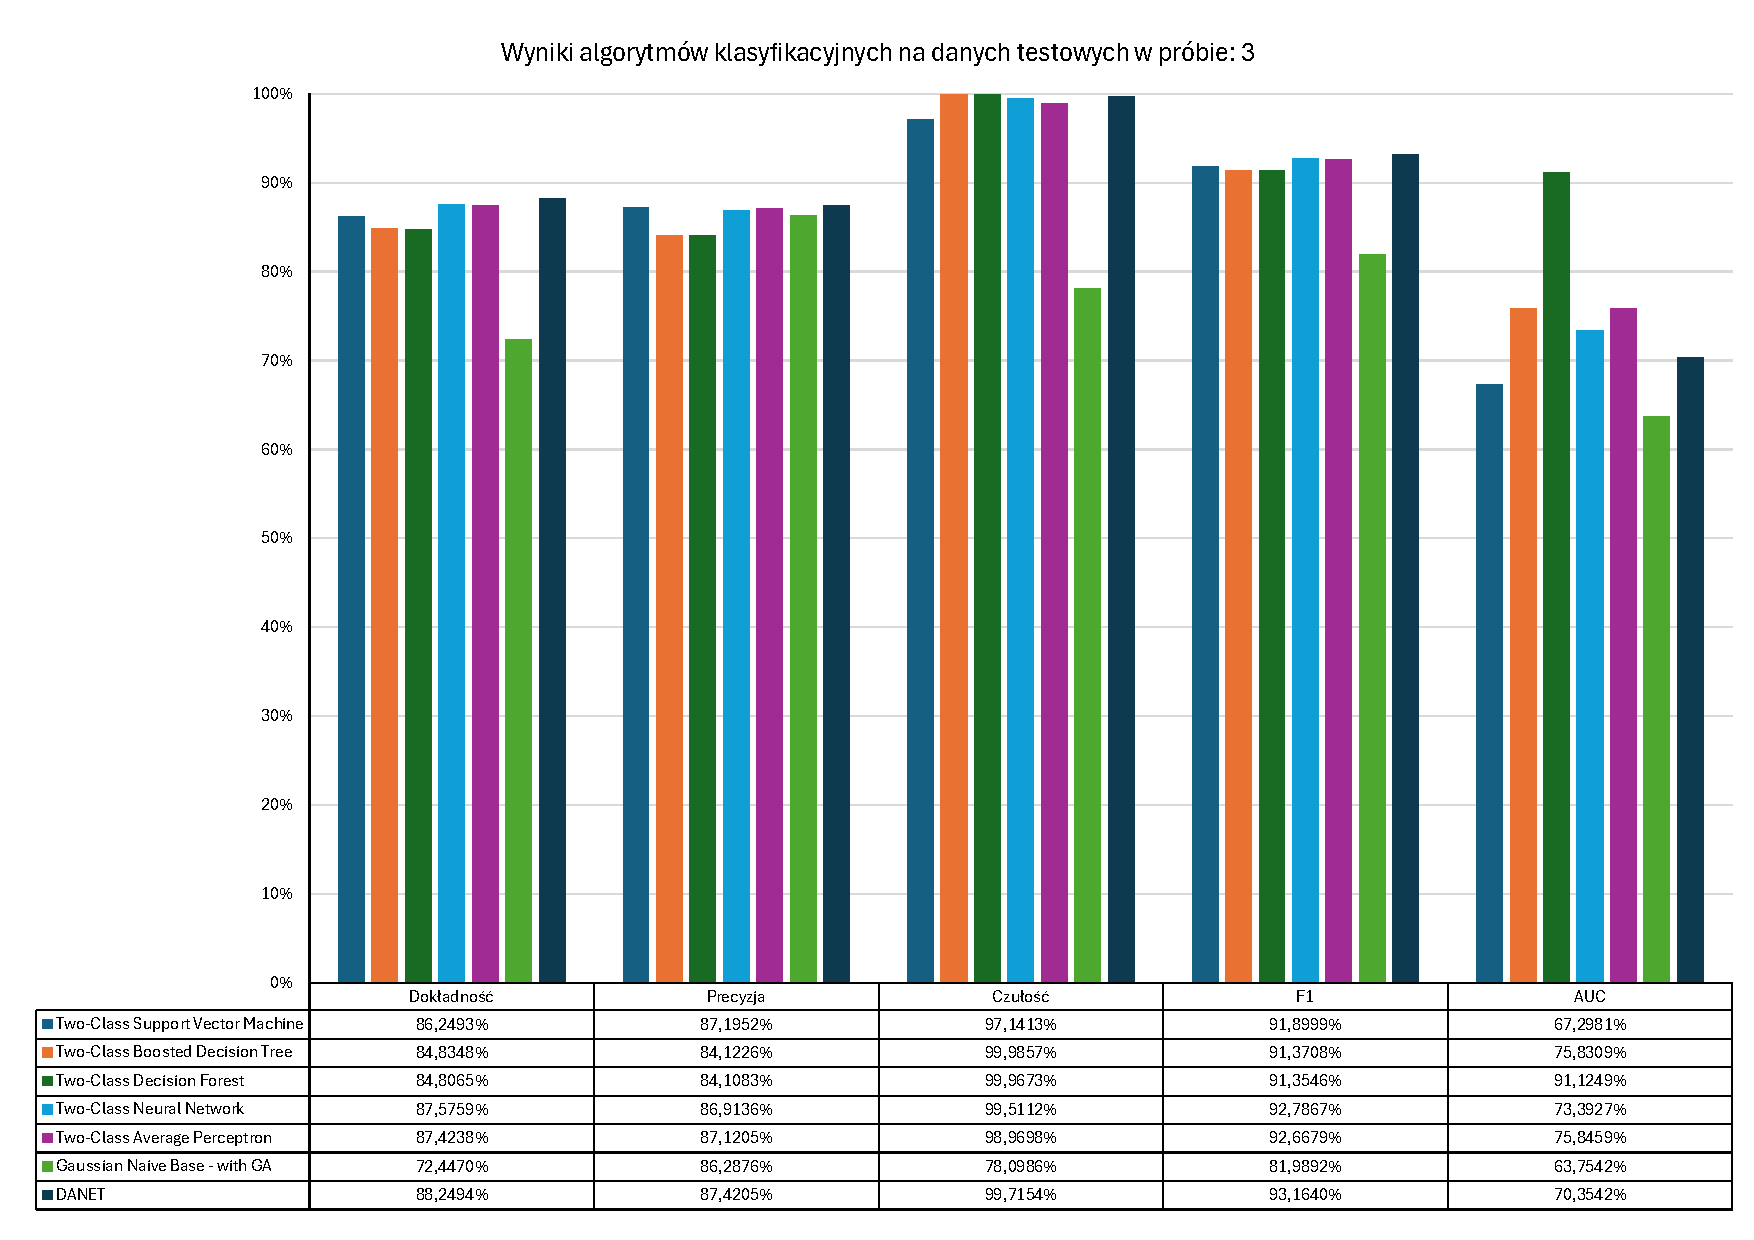
\includegraphics[height=0.8\textwidth]{images/predict_result_3}
        \captionsource{Wyniki testów algorytmów klasyfikacyjnych na danych testowych dla próby 3}{Opracowanie własne}
        \label{fig:predict-result3}
    \end{figure}
    \vfill
\end{landscape}


\section{Porównanie uzyskanych wyników między algorytmami}
Aby uzyskać realne wyniki podczas porównywania poszczególnych algorytmów zastosowano zbiór treningowy opisany w \refsource{tabeli}{tab:trening-data-label} oraz zbiór testowy opisany w \refsource{tabeli}{tab:res-test}.

\subsection{Wyniki dopasowania}
Najlepszy wynik dopasowania dla danych testowych uzyskał algorytm \textit{DANet}, który poprawnie rozpoznał $88,2494\%$ próbek.\ Najgorszy wynik uzyskał algorytm \textit{GAGNB} z dopasowaniem w zbiorze $[72,4470\%; 73,8269\%; 76,2585\%]$.\ Dla próby treningowej najlepszy wynik uzyskał \textit{Two-Class Boosted Decision Tree} z wynikiem $100,00\%$, a najgorszy \textit{GAGNB} z wynikiem $91,4271\%$.\ Wyniki dopasowania dla poszczególnych prób zostały przedstawione na \refsource{tabeli}{tab:acc-res} oraz na \refsource{wykresie}{fig:acc-res}.

\begin{table}[H]
    \centering
    \captionsourceb{Wynik dopasowania algorytmów.}{Kolorem zielonym określono najlepszy wynik w kolumnie.\ Kolorem czerwonym określono najgorszy wynik w kolumnie.}{Opracowanie własne}
    \resizebox{\textwidth}{!}{%
        \begin{NiceTabular}{|l|r|r|r||r|}[hvlines]
            & \multicolumn{4}{c|}{\textbf{Wynik dopasowania}} \\
            \textbf{Algorytm}                & \textbf{Próba Treningowa}                  & \textbf{Próba 1}                  & \textbf{Próba 2}                  & \textbf{Próba 3}             \\
            Two-Class Support Vector Machine & $99,9167\%$ & $86,2493\%$ & $86,2493\%$ & $86,2493\%$ \\
            Two-Class Boosted Decision Tree & \cellcolor{lightgreen}$100,0000\%$ & $84,8348\%$ & $84,8348\%$ & $84,8348\%$ \\
            Two-Class Decision Forest & $99,9956\%$ & $84,8065\%$ & $84,8065\%$ & $84,8065\%$ \\
            Two-Class Neural Network & $99,8401\%$ & $87,5759\%$ & $87,5759\%$ & $87,5759\%$ \\
            Two-Class Average Perceptron & $99,3834\%$ & $87,4238\%$ & $87,4238\%$ & $87,4238\%$ \\
            Gaussian Naive Base - with GA & \cellcolor{lightred}$91,4271\%$ & \cellcolor{lightred}$76,2585\%$ & \cellcolor{lightred}$73,8269\%$ & \cellcolor{lightred}$72,4470\%$ \\
            DANET & $99,8893\%$ & \cellcolor{lightgreen}$88,2494\%$ & \cellcolor{lightgreen}$88,2494\%$ & \cellcolor{lightgreen}$88,2494\%$ \\
        \end{NiceTabular}%
    }
    \label{tab:acc-res}
\end{table}

\begin{figure}[H]
    \centering
    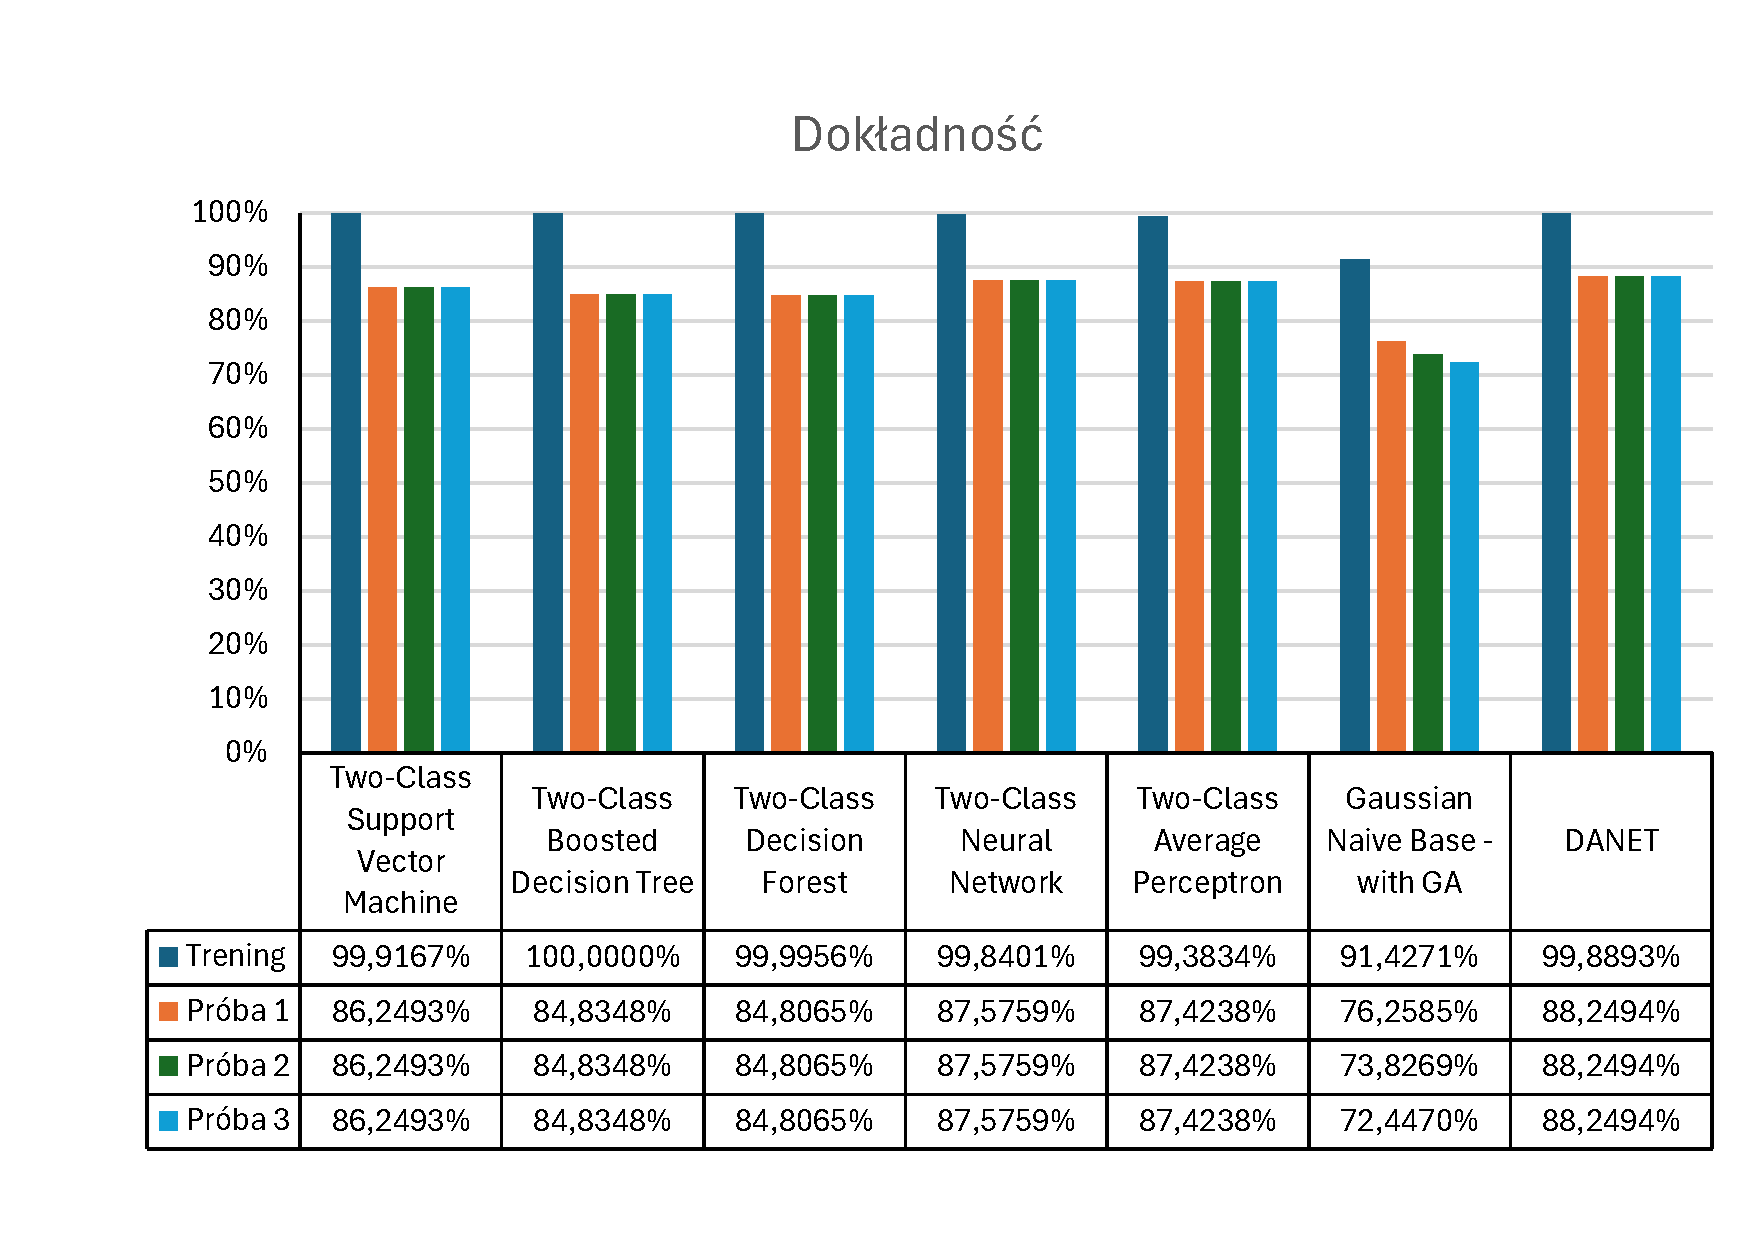
\includegraphics[width=\textwidth]{images/acc-res}
    \captionsource{Dokładność algorytmów}{Opracowanie własne}
    \label{fig:acc-res}
\end{figure}

\subsection{Wyniki precyzji}
Najlepszy wynik precyzji dla danych testowych uzyskał algorytm \textit{DANet} ($87,4205\%$).\ Najgorszy wynik uzyskał algorytm \textit{Two-Class Decision Forest} ($84,1084\%$).\ Algorytm \textit{GAGNB} uzyskał wyniki: ($[85,0422\%; , 85,4461\%; 86,2876\%]$).\  Dla próby treningowej najlepszy wynik uzyskał \textit{Two-Class Boosted Decision Tree} ($100,00\%$), a najgorszy \textit{GAGNB} ($94,2285\%$).\ Wyniki precyzji dla poszczególnych prób zostały przedstawione w \refsource{tabeli}{tab:acc-prec} oraz na wykresie \refsource{wykresie}{fig:prec-res}.

\begin{table}[H]
    \centering
    \captionsourceb{Wynik precyzji algorytmów.}{Kolorem zielonym określono najlepszy wynik w kolumnie.\ Kolorem czerwonym określono najgorszy wynik w kolumnie.}{Opracowanie własne}
    \resizebox{\textwidth}{!}{%
        \begin{NiceTabular}{|l|r|r|r||r|}[hvlines]
            & \multicolumn{4}{c|}{\textbf{Wynik precyzji}} \\
            \textbf{Algorytm}                & \textbf{Próba Treningowa}                  & \textbf{Próba 1}                  & \textbf{Próba 2}                  & \textbf{Próba 3}             \\
            Two-Class Support Vector Machine & $99,8742\%$ & $87,1952\%$ & $87,1952\%$ & $87,1952\%$ \\
            Two-Class Boosted Decision Tree & \cellcolor{lightgreen}$100,0000\%$ & $84,1226\%$ & $84,1226\%$ & $84,1226\%$ \\
            Two-Class Decision Forest & $99,9898\%$ & \cellcolor{lightred}$84,1083\%$ & \cellcolor{lightred}$84,1083\%$ & \cellcolor{lightred}$84,1083\%$ \\
            Two-Class Neural Network & $99,9231\%$ & $86,9136\%$ & $86,9136\%$ & $86,9136\%$ \\
            Two-Class Average Perceptron & $99,8510\%$ & $87,1205\%$ & $87,1205\%$ & $87,1205\%$ \\
            Gaussian Naive Base - with GA & \cellcolor{lightred}$94,2285\%$ & $85,4461\%$ & $85,0422\%$ & $86,2876\%$ \\
            DANET & $99,8568\%$ & \cellcolor{lightgreen}$87,4205\%$ & \cellcolor{lightgreen}$87,4205\%$ & \cellcolor{lightgreen}$87,4205\%$ \\
        \end{NiceTabular}%
    }
    \label{tab:acc-prec}
\end{table}

\begin{figure}[H]
    \centering
    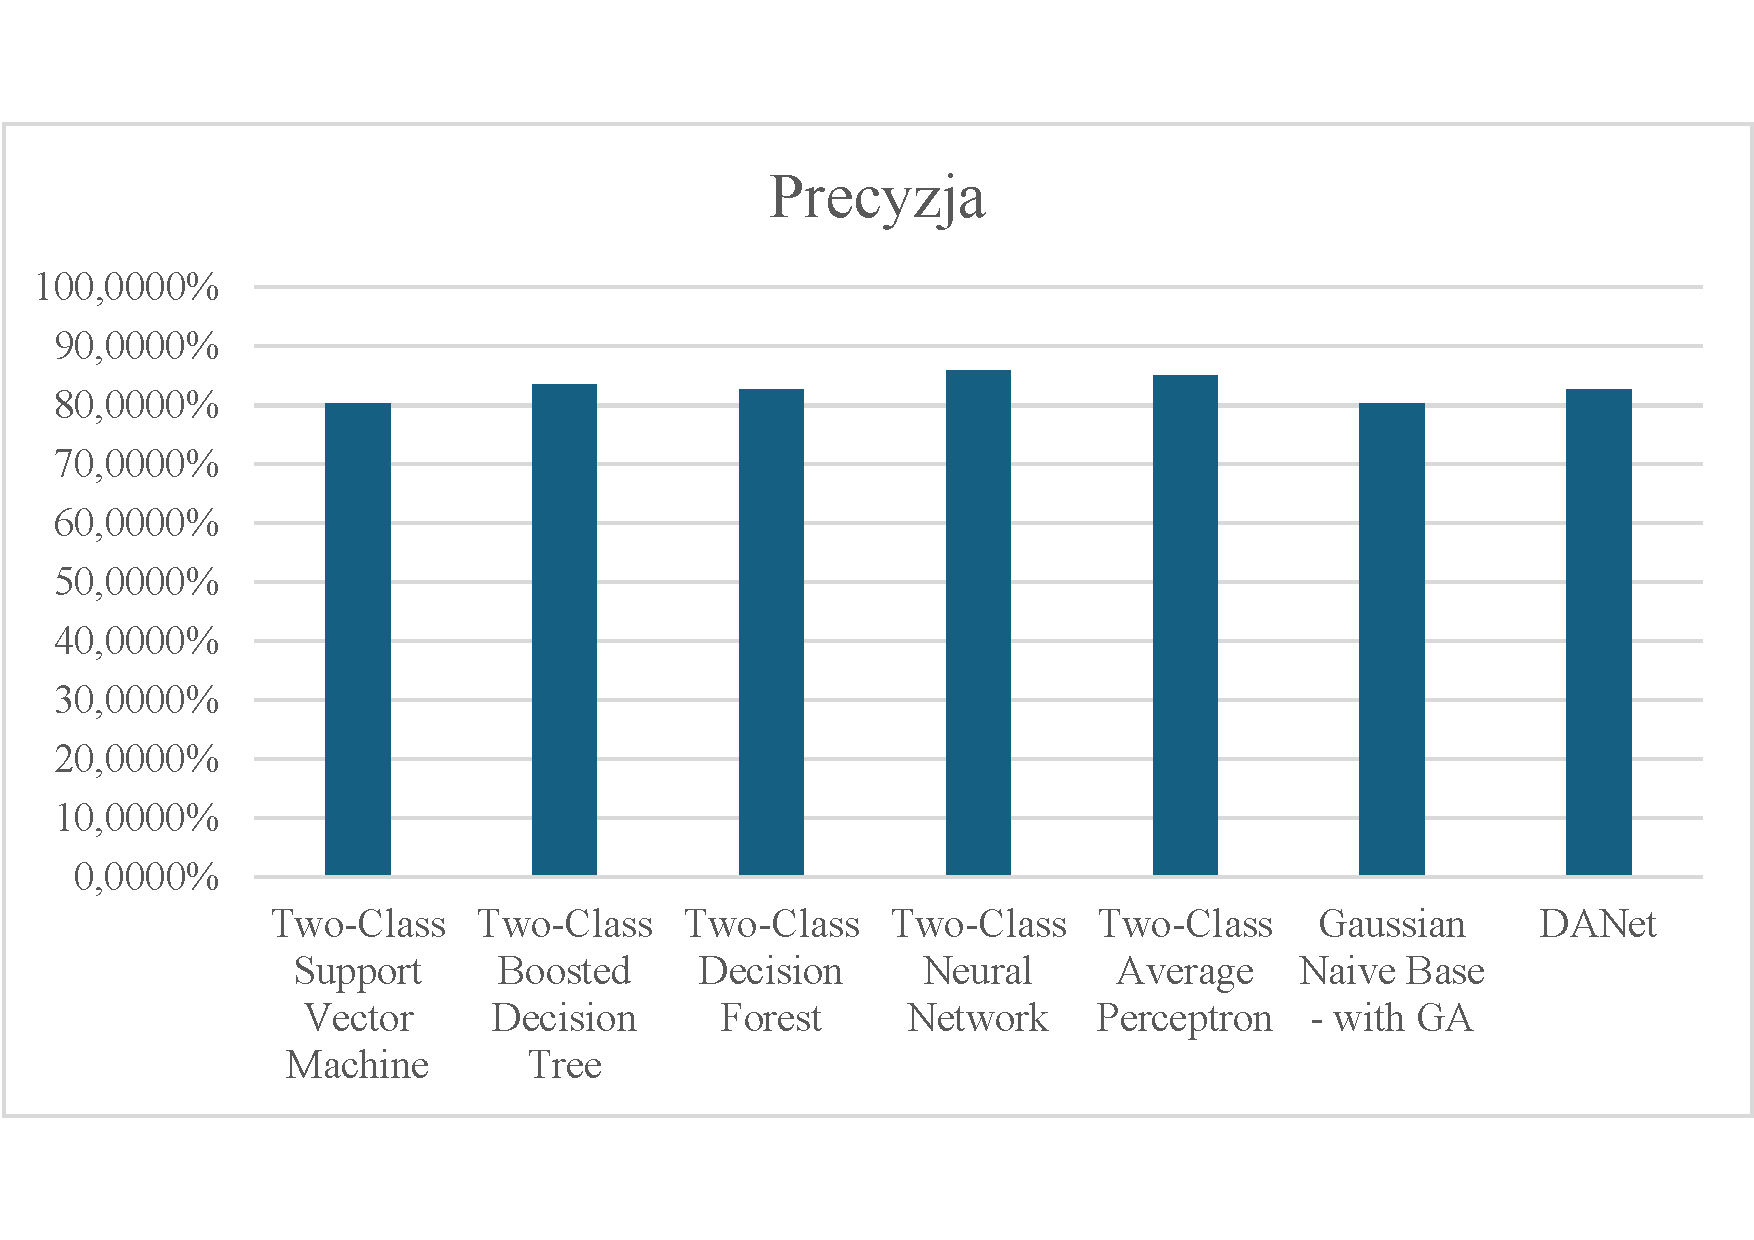
\includegraphics[width=\textwidth]{images/prec_2_wyk}
    \captionsource{Precyzja algorytmów}{Opracowanie własne}
    \label{fig:prec-res}
\end{figure}

\subsection{Wyniki czułości}
Najlepszy wynik czułości dla danych testowych uzyskał algorytm \textit{Two-Class Bosted Decision Tree} ($99,9857\%$).\ Najgorszy wynik uzyskał algorytm \textit{GAGNB} z wynikami należącymi do zbioru $[78,0986\%; 81,7923\%; 84,8940\%]$.\  Dla próby treningowej najlepszy wynik uzyskał \textit{Two-Class Boosted Decision Tree} oraz \textit{Two-Class Decision Forest} ($100,00\%$), a najgorszy \textit{Gaussian Naive Bayes - with GA} ($85,4275\%$).\ Wyniki czułości dla poszczególnych prób zostały przedstawione w \refsource{tabeli}{tab:acc-rec} oraz na wykresie \refsource{wykresie}{fig:rec-res}.

\begin{table}[H]
    \centering
    \captionsourceb{Wynik czułości algorytmów.}{Kolorem zielonym określono najlepszy wynik w kolumnie.\ Kolorem czerwonym określono najgorszy wynik w kolumnie.}{Opracowanie własne}
    \resizebox{\textwidth}{!}{%
        \begin{NiceTabular}{|l|r|r|r||r|}[hvlines]

            & \multicolumn{4}{c|}{\textbf{Wynik czułości}} \\
            \textbf{Algorytm}                & \textbf{Próba Treningowa}                  & \textbf{Próba 1}                  & \textbf{Próba 2}                  & \textbf{Próba 3}             \\
            Two-Class Support Vector Machine & $99,9335\%$ & $97,1413\%$ & $97,1413\%$ & $97,1413\%$ \\
            Two-Class Boosted Decision Tree & \cellcolor{lightgreen}$100,0000\%$ & \cellcolor{lightgreen}$99,9857\%$ & \cellcolor{lightgreen}$99,9857\%$ & \cellcolor{lightgreen}$99,9857\%$ \\
            Two-Class Decision Forest & \cellcolor{lightgreen}$100,0000\%$ & $99,9673\%$ & $99,9673\%$ & $99,9673\%$ \\
            Two-Class Neural Network & $99,7073\%$ & $99,5112\%$ & $99,5112\%$ & $99,5112\%$ \\
            Two-Class Average Perceptron & $98,7229\%$ & $98,9698\%$ & $98,9698\%$ & $98,9698\%$ \\
            Gaussian Naive Base - with GA & \cellcolor{lightred}$85,4275\%$ & \cellcolor{lightred}$84,8940\%$ & \cellcolor{lightred}$81,7923\%$ & \cellcolor{lightred}$78,0986\%$ \\
            DANET & $99,8874\%$ & $99,7154\%$ & $99,7154\%$ & $99,7154\%$ \\
        \end{NiceTabular}%
    }
    \label{tab:acc-rec}
\end{table}

\begin{figure}[H]
    \centering
    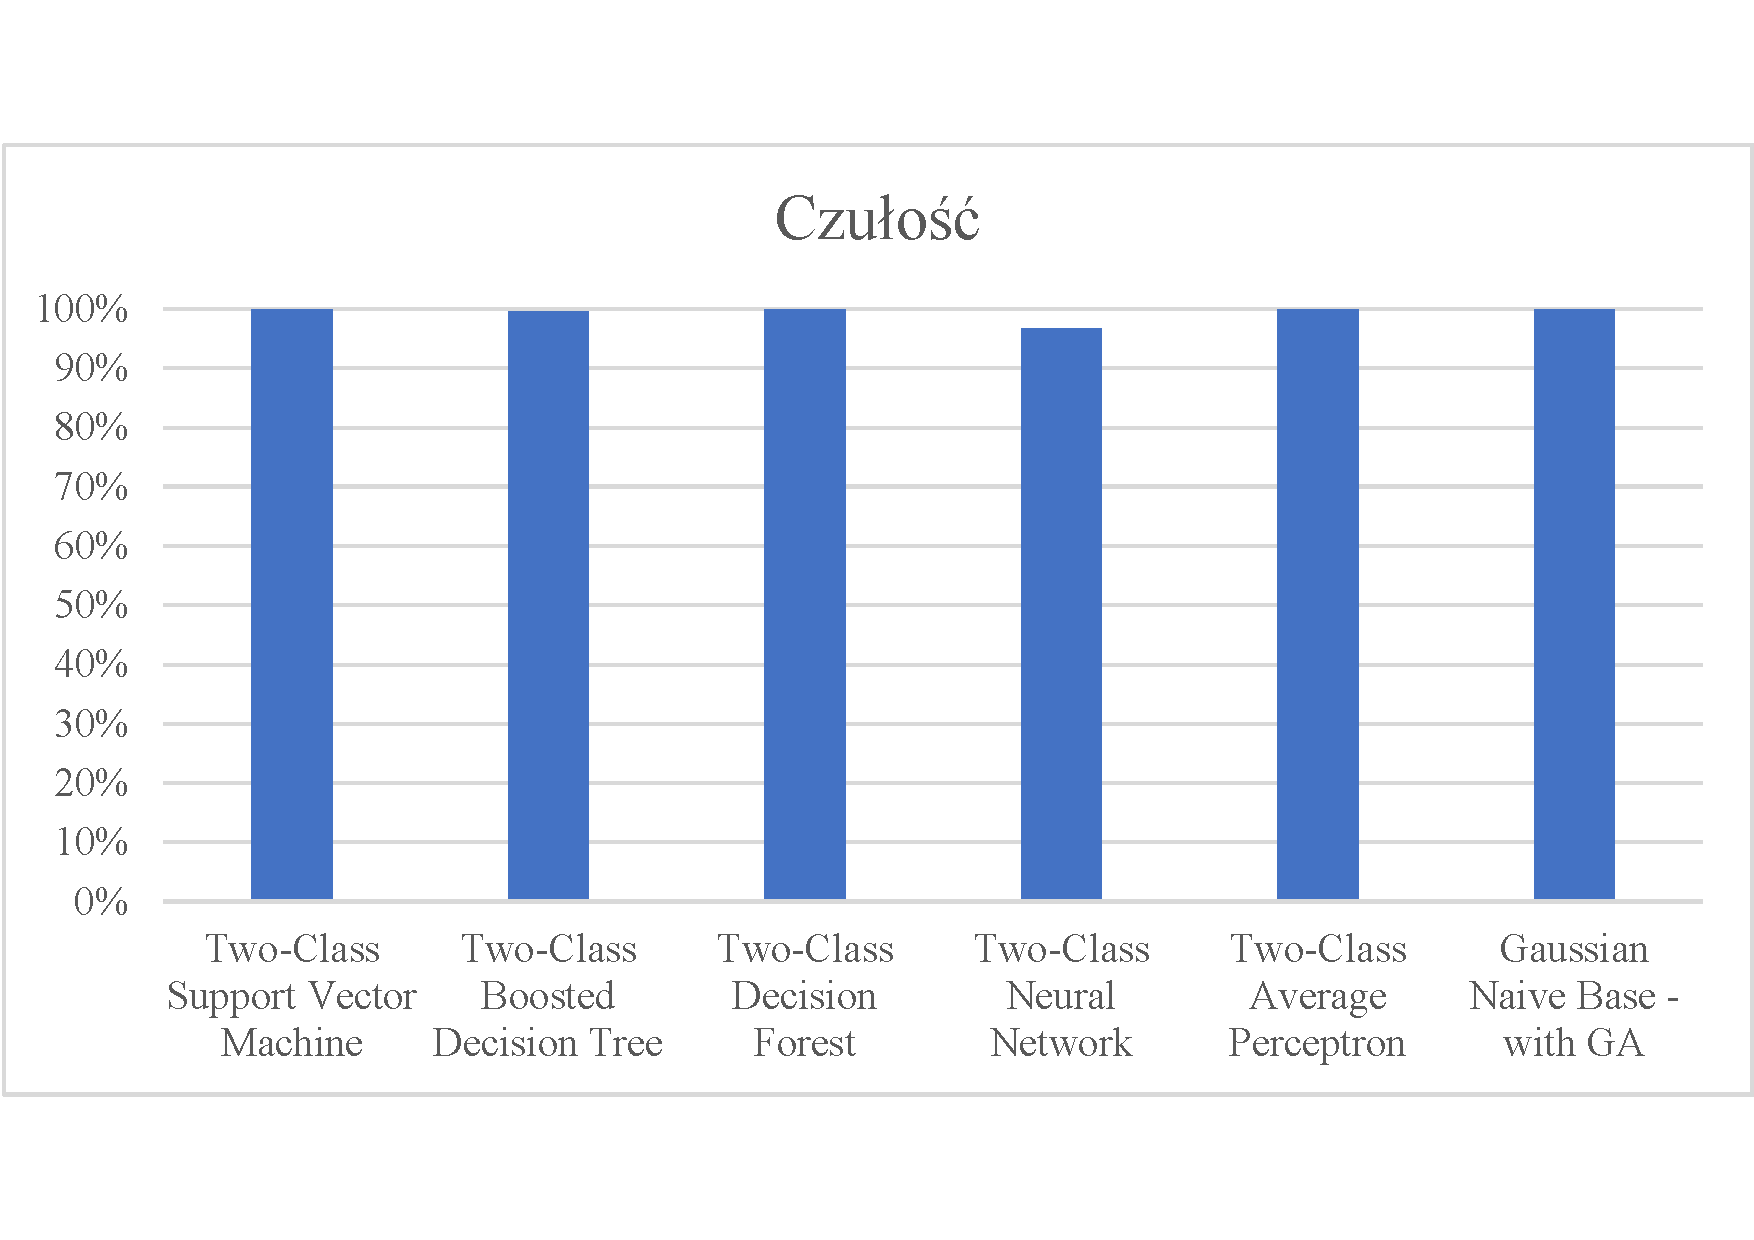
\includegraphics[width=\textwidth]{images/rec-res}
    \captionsource{Czułość algorytmów}{Opracowanie własne}
    \label{fig:rec-res}
\end{figure}

\subsection{Wyniki F1}
Najlepszy wynik F1 dla danych testowych uzyskał algorytm \textit{DANet} ($93,1640\%$).\ Najgorszy wynik uzyskał algorytm \textit{GAGNB} ($[81,9892\%; 83,3856\%; 85,1692\%]$).\ Dla próby treningowej najlepszy wynik uzyskał \textit{Two-Class Boosted Decision Tree} ($100,00\%$), a najgorszy \textit{GAGNB} ($89,6124\%$).\ Wyniki F1 dla poszczególnych prób zostały przedstawione w \refsource{tabeli}{tab:acc-f1} oraz na wykresie \refsource{wykresie}{fig:f1-res}.

\begin{table}[H]
    \centering
    \captionsourceb{Wynik F1 algorytmów.}{Kolorem zielonym określono najlepszy wynik w kolumnie.\ Kolorem czerwonym określono najgorszy wynik w kolumnie.}{Opracowanie własne}
    \resizebox{\textwidth}{!}{%
        \begin{NiceTabular}{|l|r|r|r||r|}[hvlines]

            & \multicolumn{4}{c|}{\textbf{Wynik F1}} \\
            \textbf{Algorytm}                & \textbf{Próba Treningowa}                  & \textbf{Próba 1}                  & \textbf{Próba 2}                  & \textbf{Próba 3}             \\
            Two-Class Support Vector Machine & $99,9038\%$ & $91,8999\%$ & $91,8999\%$ & $91,8999\%$ \\
            Two-Class Boosted Decision Tree & \cellcolor{lightgreen}$100,0000\%$ & $91,3708\%$ & $91,3708\%$ & $91,3708\%$ \\
            Two-Class Decision Forest & $99,9949\%$ & $91,3546\%$ & $91,3546\%$ & $91,3546\%$ \\
            Two-Class Neural Network & $99,8151\%$ & $92,7867\%$ & $92,7867\%$ & $92,7867\%$ \\
            Two-Class Average Perceptron & $99,2837\%$ & $92,6679\%$ & $92,6679\%$ & $92,6679\%$ \\
            Gaussian Naive Base - with GA & \cellcolor{lightred}$89,6124\%$ & \cellcolor{lightred}$85,1692\%$ & \cellcolor{lightred}$83,3856\%$ & \cellcolor{lightred}$81,9892\%$ \\
            DANET & $99,8721\%$ & \cellcolor{lightgreen}$93,1640\%$ & \cellcolor{lightgreen}$93,1640\%$ & \cellcolor{lightgreen}$93,1640\%$ \\
        \end{NiceTabular}%
    }
    \label{tab:acc-f1}
\end{table}

\begin{figure}[H]
    \centering
    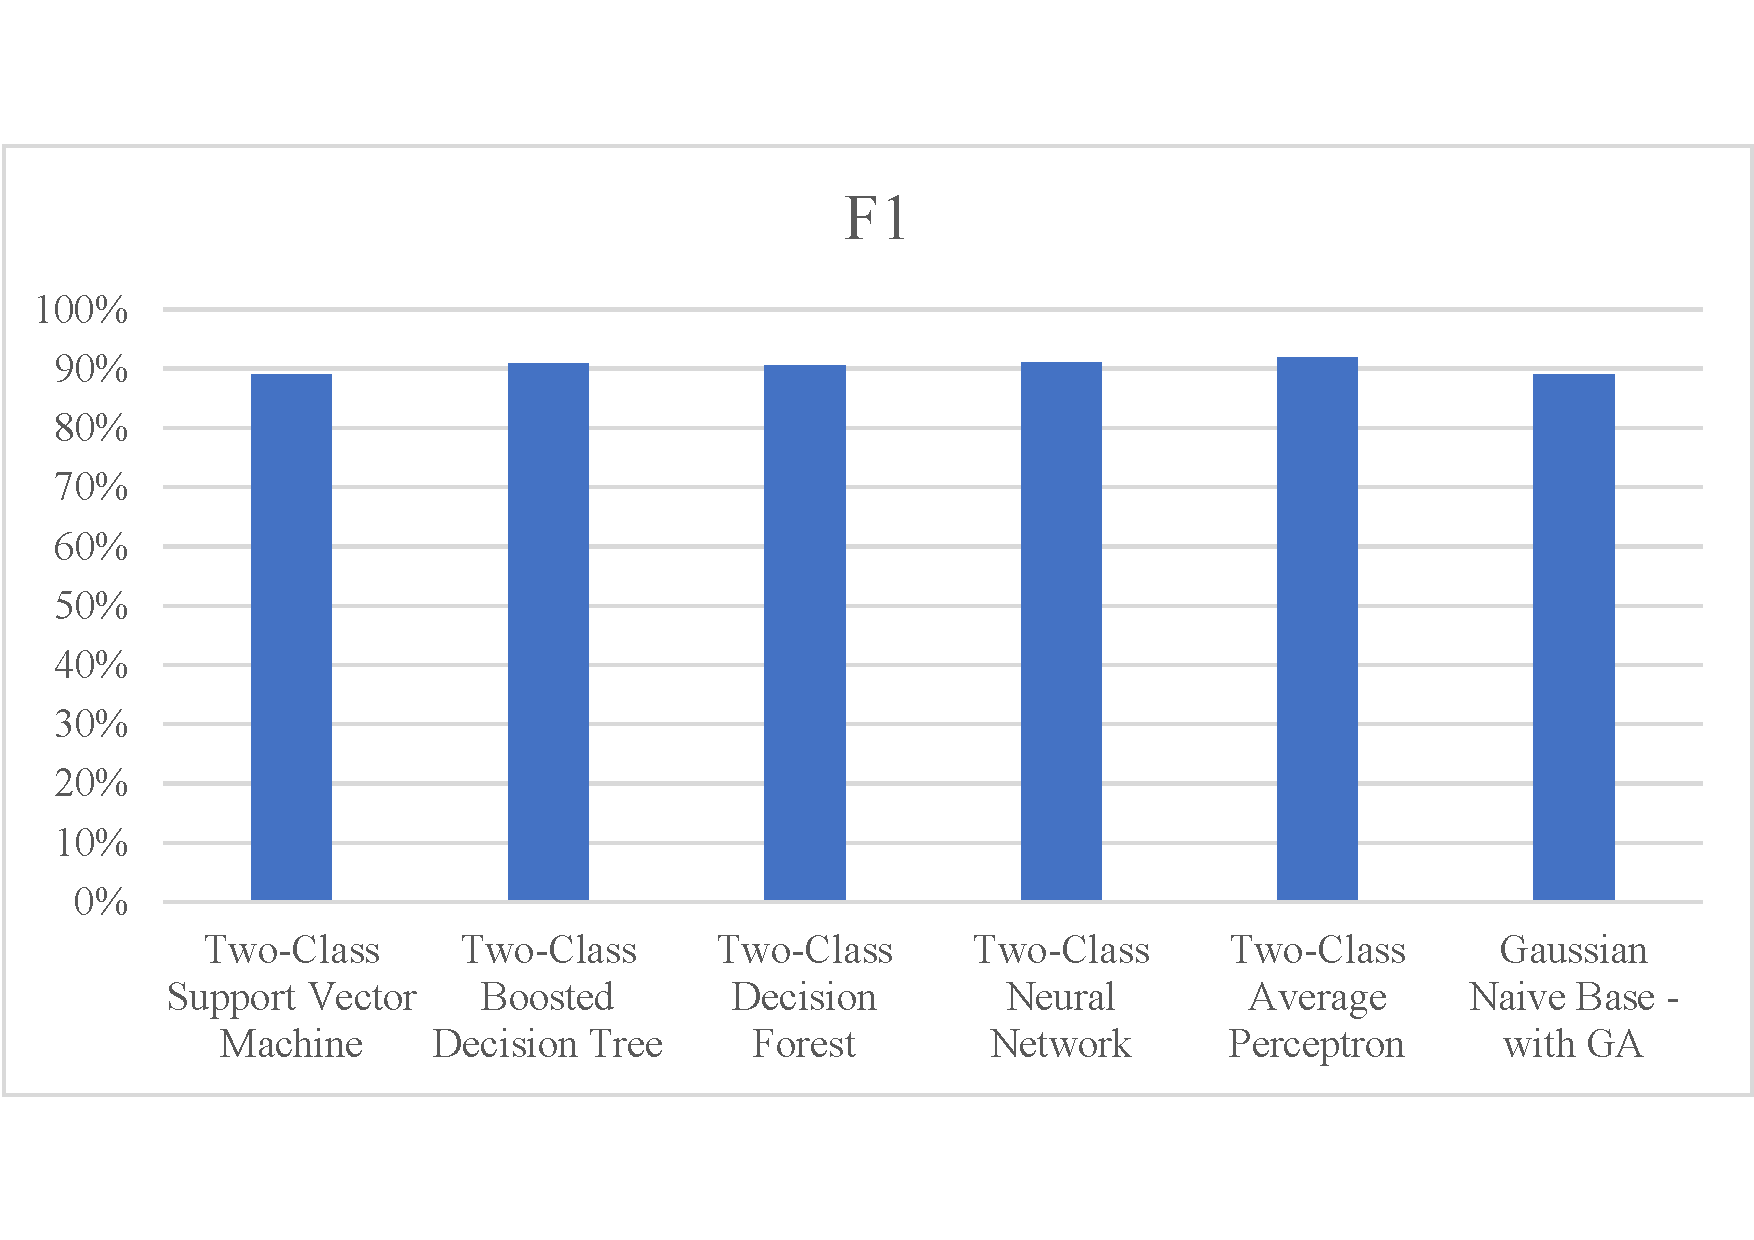
\includegraphics[width=\textwidth]{images/f1-res}
    \captionsource{F1 algorytmów}{Opracowanie własne}
    \label{fig:f1-res}
\end{figure}

\subsection{Wyniki AUC}
Najlepszy wynik precyzji dla danych testowych uzyskał algorytm \textit{Two-Class Decision Forest} ($91,1249\%$).\ Najgorszy wynik uzyskał algorytm \textit{GAGNB} ($[61,5753\%; 62,9762\%; 63,7542\%]$).\ Dla próby treningowej najlepszy wynik uzyskał \textit{Two-Class Boosted Decision Tree} oraz \textit{Two-Class Decision Forest} ($100,00\%$), a najgorszy \textit{GAGNB} ($90,7169\%$).\ Wyniki AUC dla poszczególnych prób zostały przedstawione w \refsource{tabeli}{tab:acc-auc} oraz na wykresie \refsource{wykresie}{fig:auc-res}.

\begin{table}[H]
    \centering
    \captionsourceb{Wynik AUC algorytmów.}{Kolorem zielonym określono najlepszy wynik w kolumnie.\ Kolorem czerwonym określono najgorszy wynik w kolumnie.}{Opracowanie własne}
    \resizebox{\textwidth}{!}{%
        \begin{NiceTabular}{|l|r|r|r||r|}[hvlines]
            & \multicolumn{4}{c|}{\textbf{Wynik AUC}} \\
            \textbf{Algorytm}                & \textbf{Próba Treningowa}                  & \textbf{Próba 1}                  & \textbf{Próba 2}                  & \textbf{Próba 3}             \\
            Two-Class Support Vector Machine & $99,9973\%$ & $67,2981\%$ & $67,2981\%$ & $67,2981\%$ \\
            Two-Class Boosted Decision Tree & \cellcolor{lightgreen}$100,0000\%$ & $75,8309\%$ & $75,8309\%$ & $75,8309\%$ \\
            Two-Class Decision Forest & \cellcolor{lightgreen}$100,0000\%$ & \cellcolor{lightgreen}$91,1249\%$ & \cellcolor{lightgreen}$91,1249\%$ & \cellcolor{lightgreen}$91,1249\%$ \\
            Two-Class Neural Network & $99,9974\%$ & $73,3927\%$ & $73,3927\%$ & $73,3927\%$ \\
            Two-Class Average Perceptron & $99,9762\%$ & $75,8459\%$ & $75,8459\%$ & $75,8459\%$ \\
            Gaussian Naive Base - with GA & \cellcolor{lightred}$90,7169\%$ & \cellcolor{lightred}$62,9762\%$ & \cellcolor{lightred}$61,5753\%$ & \cellcolor{lightred}$63,7542\%$ \\
            DANET & $99,9969\%$ & $70,3542\%$ & $70,3542\%$ & $70,3542\%$ \\
        \end{NiceTabular}%
    }
    \label{tab:acc-auc}
\end{table}

\begin{figure}[H]
    \centering
    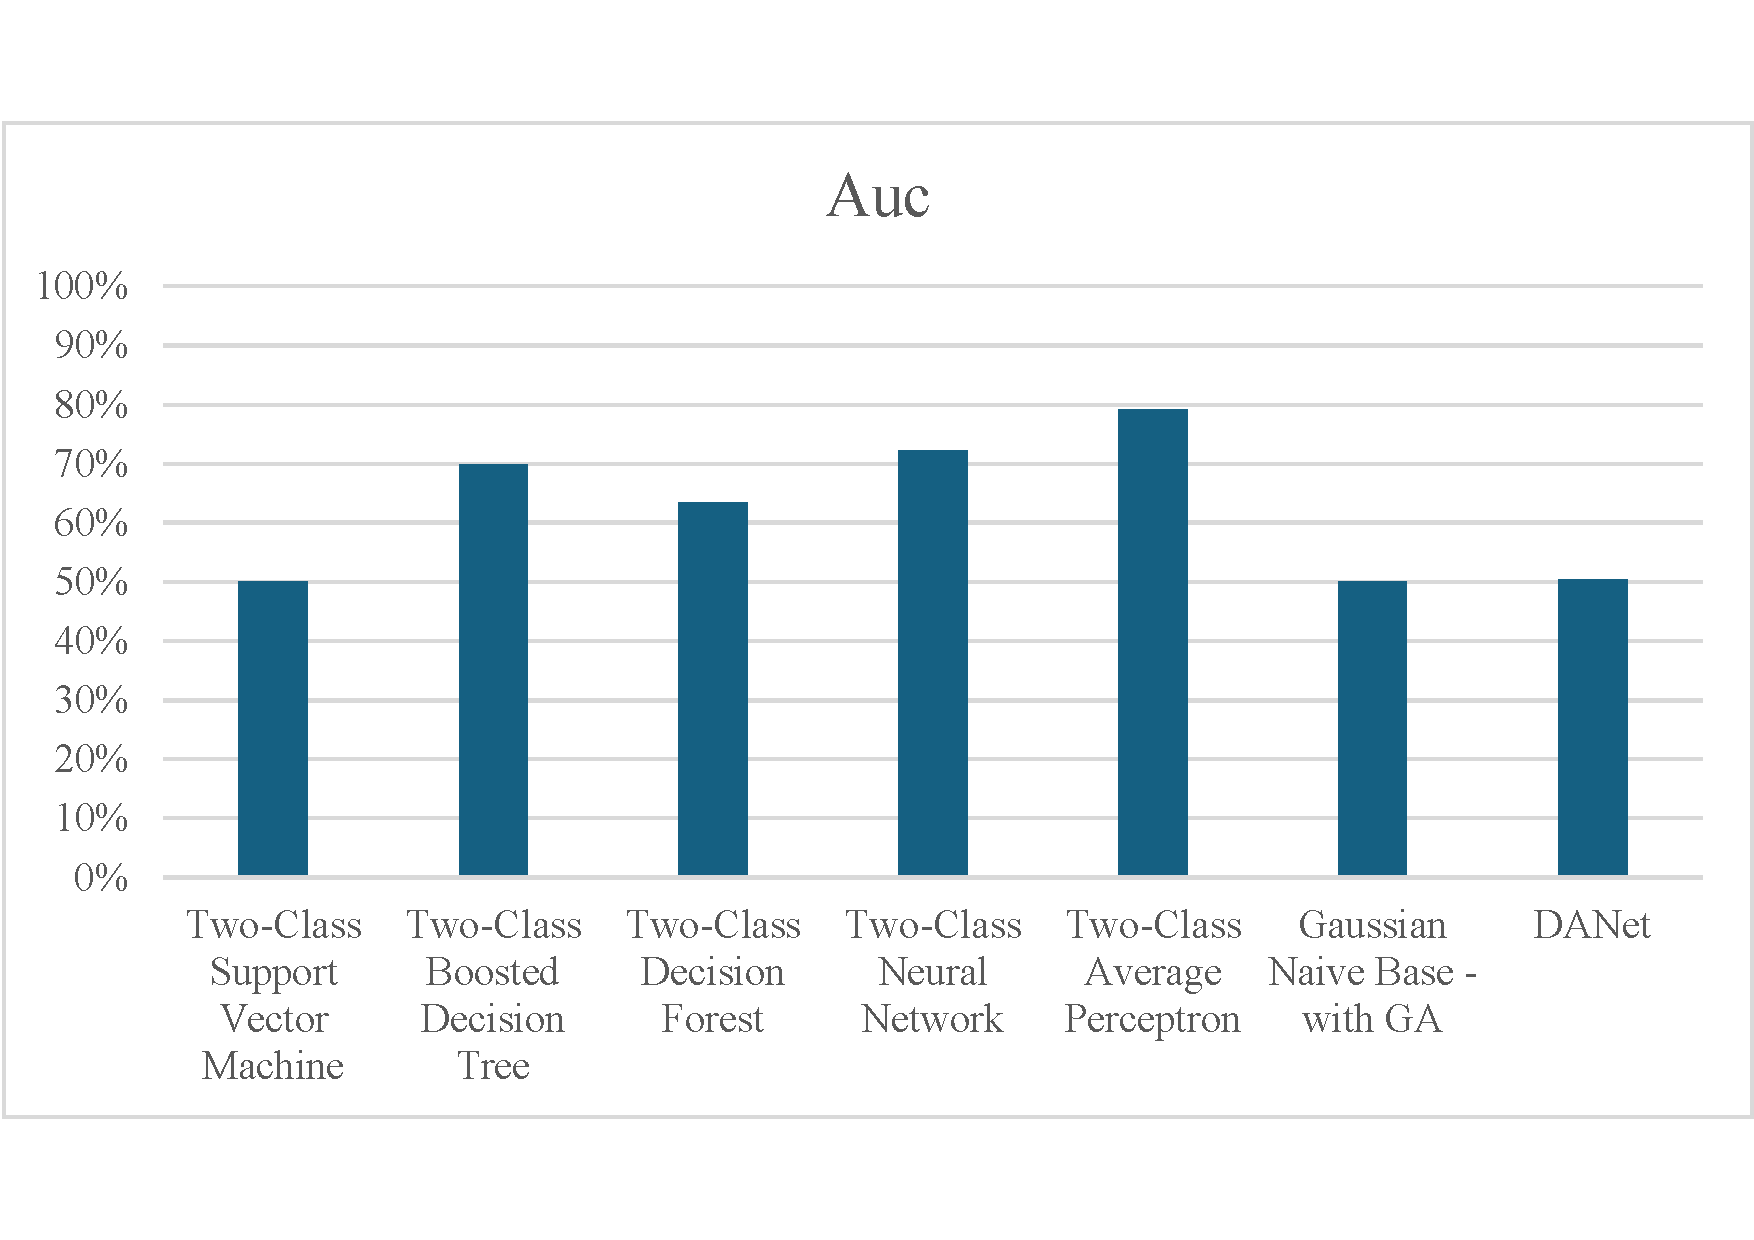
\includegraphics[width=\textwidth]{images/auc-res}
    \captionsource{AUC algorytmów}{Opracowanie własne}
    \label{fig:auc-res}
\end{figure}


\section{Analiza wyników}
Do analizy wyników wykorzystano protokół metodologii badawczej, który został opisany w \refsource{tabeli}{tab:met-bad} w \refsource{podrozdziale}{sec:met}.\ W celu weryfikacji przyjętych hipotez wykonano testy t-Studenta.\ Test t-studenta służy do analizy średniej arytmetycznej oraz odchylenia standardowego dwóch grup.\ Pozwala na rozpoznanie czy dwie grupy są różne istotnie statystycznie~\cite{tstudent}.\ Hipotezy zostały postawione dla \refsource{tabeli}{tab:acc-res}.

\begin{table}[H]
    \centering
    \captionsource{Założenia wykorzystywane do analizy statystycznej danych}{Opracowanie własne}
    \begin{tabular}{|l|c|}
        \hline
        \textbf{Założenie} & \textbf{Wartość} \\ \hline
        Przedział ufności  & $95\%$           \\ \hline
        $\alpha$           & $0,05$           \\ \hline
        Liczba elementów   & $7$              \\ \hline
    \end{tabular}
    \label{tab:stat}
\end{table}

\begin{itemize}
    \item \textbf{Hipoteza $H_0$: Nie ma istotnej różnicy pomiędzy wynikami ''dopasowania'' próby testowej i treningowej nr. 1}

    Wykorzystując statystyczny test t Studenta dla prób zależnych dla danych z \refsource{tabeli}{tab:acc-res} wyznaczono wartość:
    \begin{equation}
        \label{eq:test-t}
        t = \frac{\overline{d}}{sd_d} * \sqrt{n} = \frac{0,1358}{0,0150} * \sqrt{7} = 23,9527
    \end{equation}
    gdzie:
    \begin{itemize}
        \item $\overline{d}$ - średnia różnic w próbie
        \item $sd_d$ - odchylenie standardowe
        \item n - liczebność próby
    \end{itemize}
    \begin{table}[H]
        \centering
        \captionsource{Tabela rozkładu wartości dla t-Studenta}{\cite{Gerstman}}
        \resizebox{\textwidth}{!}{%
        \begin{tabular}{|c|l|l|l|l|l|l|l|l|l|l|}
            \hline
            \textbf{\diagbox{n}{p}} & \textbf{0,5} & \textbf{0,2} & \textbf{0,1} & \textbf{0,05} & \textbf{0,02} & \textbf{0,01} & \textbf{0,001} & \textbf{0,00001} & \textbf{0,000001} & \textbf{0,0000001} \\ \hline
            1 & 0 & 1,37638192 & 3,07768354 & 6,313751515 & 15,89454484 & 31,82052 & 31,82052 & 31830,99 & 318309,9 & 3183098,9 \\ \hline
            2 & 0 & 1,060660172 & 1,88561808 & 2,91998558 & 4,848732214 & 6,964557 & 6,964557 & 223,6034 & 707,1057 & 2236,0676 \\ \hline
            3 & 0 & 0,978472312 & 1,63774435 & 2,353363435 & 3,48190876 & 4,540703 & 4,540703 & 47,92773 & 103,2995 & 222,57159 \\ \hline
            4 & 0 & 0,940964577 & 1,53320627 & 2,131846786 & 2,998527873 & 3,746947 & 3,746947 & 23,33218 & 41,57785 & 73,985758 \\ \hline
            5 & 0 & 0,91954378 & 1,47588405 & 2,015048373 & 2,756508522 & 3,36493 & 3,36493 & 15,54685 & 24,77103 & 39,34182 \\ \hline
            6 & 0 & 0,905703285 & 1,43975575 & 1,943180281 & 2,612241847 & 3,142668 & 5,207626 & 12,03165 & 17,83031 & 26,2867 \\ \hline
            7 & 0 & 0,896029644 & 1,41492393 & 1,894578605 & 2,516752424 & 2,997952 & 2,997952 & 10,10268 & 14,24147 & 19,933902 \\ \hline
        \end{tabular}%
        }
        \label{tab:p-val}
    \end{table}
        gdzie:
        \begin{itemize}
            \item \textbf{n} - ilość punktów swobody
            \item \textbf{p} - wartość p-value
        \end{itemize}
    Następnie bazując na \refsource{tabeli}{tab:p-val} obrazującej rozkład wartości \textit{t} dla \textit{n} punktów swobody w \textit{p-value} znaleziono wartość p-value odpowiadającej otrzymanemu wynikowi.\ Dla 6 punktów swobody: $0,000001 < p-value < 0,0000001$.\ Oznacza to, że zmienna $p-value < \alpha$, dzięki czemu można odrzucić hipotezę $H_0$.\ Wyniki tej analizy określają, że widać istotne różnice pomiędzy danymi z próby testowej i treningowej.\ Największą różnicę widać w rezultacie algorytmu \textit{GAGNB}, który uzyskał w próbie testowej $76,2585\%$ dopasowania, a w próbie treningowej $91,4271\%$.\\

    \item \textbf{Hipoteza $H_0$: Nie ma istotnej różnicy pomiędzy wynikami ''dopasowania'' prób testowych}
    Korzystając z \refsource{wzoru}{eq:test-t}, wykonano obliczenia dla poszczególnych relacji przedstawionych w \refsource{tabeli}{tab:acc-p-stat}.
    \begin{equation}
        \label{eq:t-p1}
        t_1 = \frac{d_{p2p3}}{sd_{d_{p2p3}}} * \sqrt{n} = \frac{0,0019713}{0,0048287} * \sqrt{7} = 1,0801
    \end{equation}
    \begin{equation}
        \label{eq:t-p2}
        t_2 = \frac{d_{p1p2}}{sd_{p1p2}} * \sqrt{n} = \frac{0,0034737}{0,0085088} * \sqrt{7} = 1,0801
    \end{equation}
    \begin{equation}
        \label{eq:t-p3}
        t_3 = \frac{p1p3}{p1p3} * \sqrt{n} = \frac{0,0054450}{0,0133375} * \sqrt{7} = 1,0801
    \end{equation}
    gdzie:
    \begin{itemize}
        \item $\overline{d}$ - średnia różnic w próbie
        \item $sd_d$ - odchylenie standardowe
        \item $n$ - liczebność próby
        \item $p1$ - próba 1
        \item $p2$ - próba 2
        \item $p3$ - próba 3
    \end{itemize}

    Wyniki równań zostały przedstawione w \refsource{tabeli}{tab:acc-p-stat} w kolumnie \textit{wartość t}.

    \begin{table}[H]
        \centering
        \captionsource{Wyniki testu t-Studenta dla poszczególnych prób testowych}{Opracowanie własne}
        \begin{tabular}{|c|c|r|c|P{30mm}|}
            \hline
            \multicolumn{5}{|c|}{$H_0$ Brak istotnych różnic między wynikami dla $\alpha = 0,05$} \\ \hline
            \textbf{L.p.} & \textbf{Relacja}                  & \textbf{Wartość \textit{t}} & \textbf{P-value}      & \textbf{Rezultat}                                 \\\hline
            \textbf{1}    & Próba 2 $\leftrightarrow$ Próba 3 & $1,801$                         & $0,2 < p-value < 0,5$                 & $p-value > \alpha$ \newline Brak istotnych różnic \\ \hline
            \textbf{2}    & Próba 2 $\leftrightarrow$ Próba 1 & $1,0801$                    & $0,2 < p-value < 0,5$ & $p-value > \alpha$ \newline Brak istotnych różnic \\ \hline
            \textbf{3}    & Próba 3 $\leftrightarrow$ Próba 1 & $1,0801$                    & $0,2 < p-value < 0,5$ & $p-value > \alpha$ \newline Brak istotnych różnic \\ \hline
        \end{tabular}
        \label{tab:acc-p-stat}
    \end{table}
    Za pomocą testu t Studenta dla prób zależnych określono porównano dane w próbach testowych z \refsource{tabeli}{tab:acc-res}.\ Uzyskane wyniki, przedstawione w \refsource{tabeli}{tab:acc-p-stat}, pozwalają zachować Hipotezę $H_0$, stwierdzającą, że pomiędzy danymi w poszczególnych próbach testowych nie ma istotnych różnic. \\

    \item \textbf{Hipoteza $H_0$: Wynik dopasowania algorytmów w \textit{Próbie 1} nie przekracza dolnej granicy przedziału ufności}
    Za pomocą \textbf{równań}~\ref{eq:uf},~\ref{eq:uf-d} obliczono wartość ufności dla zbioru wyników dopasowań w Próbie 1 oraz dolną granicę ufności.

    \begin{equation}
        \label{eq:uf}
        u = 1,96 * \frac{\sigma}{\sqrt{n}} = 1,96*\frac{0,0411}{\sqrt{7}} = 0,0346
    \end{equation}
    \begin{equation}
        \label{eq:uf-d}
        u_d = \overline{X} - u = 0,8506 - 0,0346 = 0,816
    \end{equation}
    gdzie:
    \begin{itemize}
        \item $u$ - ufność
        \item $u_d$ - dolna granica przedziału ufności
        \item $\overline{X}$ - średnia
        \item $1,96$ - kwantyl rozkładu normalnego standardowego dla $\alpha/2 \rightarrow 2,5\%$
        \item $\sigma$ - odchylenie standardowe
        \item $n$ - liczebność próby
    \end{itemize}

    Ufności dla dokładności algorytmów wyrażona w procentach wyniosła $3,46 p.p.$ dla $\alpha = 0.05$.\ Biorąc pod uwagę ten fakt, można stwierdzić, że dokładność algorytmu GAGNB jest poniżej dolnej granicy.\ Dolna granica przedziału ufności wyrażona w procentach wynosi $81,6\%$, zaś GAGNB uzyskał $76,2585\%$.\ Oznacza to, że można odrzucić $H_0$, ponieważ jeden algorytm przekracza dolny próg granicy ufności. \\
\end{itemize}

Analiza wyników wykazała, że algorytm utworzony w ramach pracy inżynierskiej~\cite{Blyszcz2022}, wypada słabo w porównaniu z algorytmami dostarczonymi przez platformę Microsoft Azure.\ Jego dokładność odstaje od dokładności uzyskanych przez pozostałe algorytmy.\ Zostało to przedstawione w \refsource{tabeli}{tab:acc-res}.\ Wyniki uzyskane przez algorytm \textit{Gaussian Naive Bayes - with GA} wynoszą $[72,4470\%; 73,8269\%; 76,2585\%]$.\ Wyniki te są słabsze o około 12-16 p.p. od wyniku uzyskanego przez algorytm DANet.\ Bazując na \textbf{tabelach}~\textbf{\ref{tab:trening-data-label}}~\textbf{\ref{tab:res-test}} różnica wielkości danych treningowych oraz testowych wyniosła:
\begin{itemize}
    \item 225805 wierszy w danych treningowych
    \item 2830743 wierszy w danych testowych
\end{itemize}

Doświadczenie to pokazuje, że wciąż należy próbować tworzyć wydajniejsze i dokładniejsze rozwiązania.\ Nie zaprzecza faktu iż rozwiązania ogólnie dostępne są często wystarczające i dużo tańsze w zastosowaniu i implementacji w porównaniu do całego procesu tworzenia rozwiązań autorskich.